\documentclass[aspectratio=169]{beamer}
\usepackage{listings}
\usepackage[utf8]{inputenc}
\usepackage[T1]{fontenc}
\usepackage{subfigure}
\usepackage{xcolor}
\usepackage{tikz}
\usepackage{tikzscale}
\usepackage{animate}
\usetikzlibrary{decorations.pathreplacing}
\usetikzlibrary{calc}
\usetikzlibrary{shapes,snakes}
\usetikzlibrary{patterns}
% BIBLIOGRAPHY
\usepackage[style=numeric, 
            backend=biber,
            giveninits=true,
            maxbibnames=9]{biblatex}
\setbeamertemplate{bibliography item}{\insertbiblabel}
\addbibresource{bibliography.bib}
\preto\fullcite{\AtNextCite{\defcounter{maxnames}{99}}}
% MATH
\usepackage{amsmath,amsfonts,amssymb,amsthm} % For math equations, theorems, symbols, etc
\usepackage{mathtools}
\usepackage{dsfont}
\DeclareMathOperator*{\argmax}{arg\,max}



%
% TIKZ equation terms' highlight
%% https://tex.stackexchange.com/questions/458694/highlighting-part-of-equation-with-text-underneath
\usetikzlibrary{tikzmark}
\tikzset{upper node/.style={inner sep=2,fill=blue!10},
lower node/.style={inner sep=1,ellipse,fill=blue!3},
ul line/.style={thick,blue!20},
upper/.code={\tikzset{upper node/.append style={#1}}},
lower/.code={\tikzset{lower node/.append style={#1}}},
line/.code={\tikzset{ul line/.append style={#1}}},
}
\newcounter{HighLight}
\newcommand{\highlight}[3][]{%
\stepcounter{HighLight}
\tikzset{#1}
\underset{\underset{\displaystyle\makebox[0pt]{\text{\tikzmarknode[lower node]{below-\theHighLight}{%
#3}}}}{\phantom{!}}}{\tikzmarknode[upper node]{above-\theHighLight}{#2}}
\tikz[overlay,remember picture]{\draw[ul line] (above-\theHighLight) --
(below-\theHighLight);}
}




\definecolor{codegreen}{rgb}{0,0.6,0}
\definecolor{codegray}{rgb}{0.5,0.5,0.5}
\definecolor{codepurple}{rgb}{0.58,0,0.82}
\definecolor{backcolour}{rgb}{0.95,0.95,0.92}
\lstdefinestyle{mystyle}{
    backgroundcolor=\color{backcolour},
    commentstyle=\color{codegreen},
    keywordstyle=\color{magenta},
    numberstyle=\tiny\color{codegray},
    stringstyle=\color{codepurple},
    basicstyle=\ttfamily\footnotesize,
    breakatwhitespace=false,
    breaklines=true,
    captionpos=b,
    keepspaces=true,
    numbers=left,
    numbersep=5pt,
    showspaces=false,
    showstringspaces=false,
    showtabs=false,
    tabsize=2
}
\lstset{style=mystyle}


\title{NFV Orchestration in Edge and Fog Scenarios}
\date{26\textsuperscript{th} October, 2021}
\author{
    {\footnotesize \textit{student}}: \! \! \! J. Martín-Pérez\\
    {\footnotesize \textit{supervisor}}: C. J. Bernardos\\
    \vspace{2em}
    \footnotesize{\textit{contact}: \href{mailto:jmartinp@it.uc3m.es}{jmartinp@it.uc3m.es}}
}

\usetheme{uc3m}
% Don't show [2/17], rather show [2]
\setbeamertemplate{footline}{%
\raisebox{5pt}{\makebox[\paperwidth]{\hfill\makebox[10pt]{\scriptsize\insertframenumber\hspace{1em}}}}}

\begin{document}

\begin{frame}[plain]
\titlepage
\end{frame}

\setcounter{framenumber}{0}


% MOTIVATION WITH POINTS ON SIDE
%%% \begin{frame}
%%%     \frametitle{Motivation}
%%% 
%%%     \begin{minipage}{.5\textwidth}
%%%         \only<6>{\color{gray}}
%%%         To assess NFV orchestration in Edge \& Fog:\pause
%%%         \begin{enumerate}
%%%             \item\only<6>{\color{gray}} graphs to represent 5G infra. \pause
%%%             \item\only<6>{\color{gray}} service @local or @federated infra. \pause
%%%             \item\only<6>{\color{gray}} embed service in the infra. \pause
%%%             \item\only<6>{\color{gray}} scale the embedded service \pause
%%%         \end{enumerate}
%%%     \end{minipage}
%%%     \only<6>{
%%%         \begin{minipage}{.45\textwidth}
%%%             \begin{enumerate}
%%%                 \item Generation of 5G infrastructure graphs
%%%                 \item NFV orchestration in federated environments
%%%                 \item NFV orchestration in 5G networks: OKpi
%%%                 \item Scaling of V2N services: a study case
%%%             \end{enumerate}
%%%         \end{minipage}
%%%     }
%%% \end{frame}

\begin{frame}
    \frametitle{Introduction}

    \textit{``Service orchestration is the process of designing, creating, delivering, and monitoring service offerings in an automated way.''} -- Ericsson

\end{frame}



\begin{frame}
    \frametitle{Introduction}
    \only<1>{
        \begin{figure}
            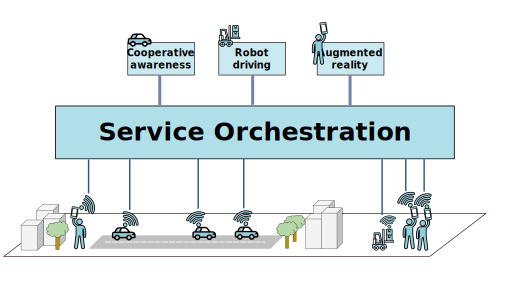
\includegraphics[width=.8\textwidth]{img/big-picture-start.pdf}
            \caption{Orchestration of three services.}
        \end{figure}
    }%
    \only<2>{
        \begin{minipage}{0.4\textwidth}
            Service Orchestration:
            \begin{itemize}
                \item design network
                \item where services run?
                \item deliver to users
                \item monitor/scale service
            \end{itemize}
        \end{minipage}
        \begin{minipage}{0.59\textwidth}
            \begin{figure}
                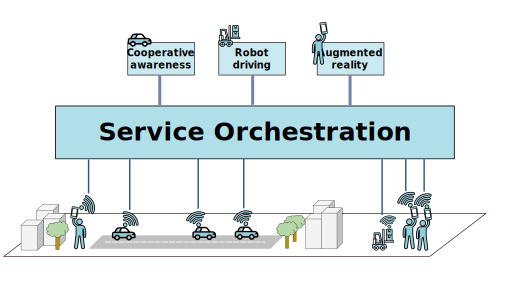
\includegraphics[width=\textwidth]{img/big-picture-start.pdf}
                \caption{Orchestration of three services.}
            \end{figure}
        \end{minipage}

    }
\end{frame}




%% \begin{frame}
%%     \frametitle{Motivation}
%% 
%%     To assess orchestration \footnote{The presentation focuses on the main thesis contributions.}:
%%     \begin{enumerate}
%%         \item design 5G infrastructure
%%         \item create service @local or @federated infrastructure
%%         \item embed service in the infrastructure
%%         \item monitor/scale the embedded service
%%     \end{enumerate}
%% \end{frame}





\begin{frame}
    \frametitle{Outline}
    \tableofcontents[hideallsubsections,pausesections]
\end{frame}



\section{Generation of 5G infrastructure graphs}
\subsection{Motivation}
\begin{frame}
    \frametitle{Outline}
    \tableofcontents[subsectionstyle=show/shaded/hide,sectionstyle=show/shaded]
\end{frame}


%% OLD MOTIVATION SLIDE
%% \begin{frame}
%%     \frametitle{\secname}
%%     \framesubtitle{\subsecname}
%% 
%%     \begin{figure}
%%         \centering
%%         \includegraphics[width=.8\textwidth]{img/pop-and-antennas-no-labels.pdf}
%%         \caption{Illustration of BS and PoPs in Madrid.}
%%         \label{fig:bs-pops-no-label}
%%     \end{figure}
%% \end{frame}




\begin{frame}
    \frametitle{\secname}
    \framesubtitle{\subsecname}

    \only<1-2>{
        \begin{figure}
            \centering
            \only<1>{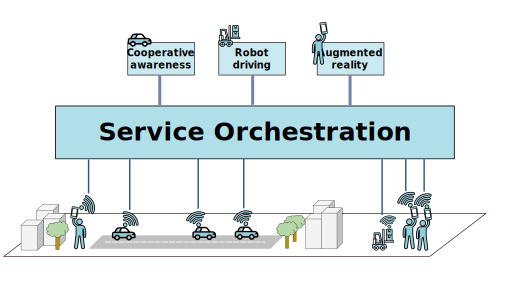
\includegraphics[width=.8\textwidth]{img/big-picture-start.pdf}}%
            \only<2>{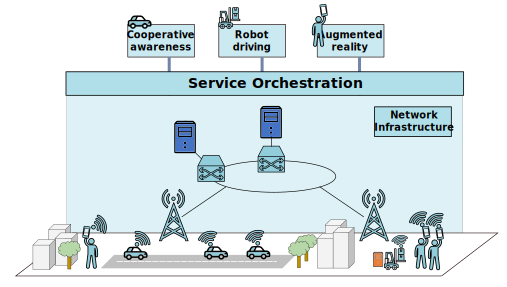
\includegraphics[width=.8\textwidth]{img/big-picture-infra-gen.pdf}}
            \caption{
                \only<2>{Network infrastructure for service providing.}
            }
            \label{fig:big-infra}
        \end{figure}
    }%
    \only<3>{
        \begin{minipage}{0.45\textwidth}
            In this part -- \textbf{location} of:
            \begin{enumerate}
                \item \textbf{BSs} for user coverage
                \item \textbf{servers} to process traffic
            \end{enumerate}
        \end{minipage}
        \begin{minipage}{0.5\textwidth}
            \begin{figure}
                \centering
                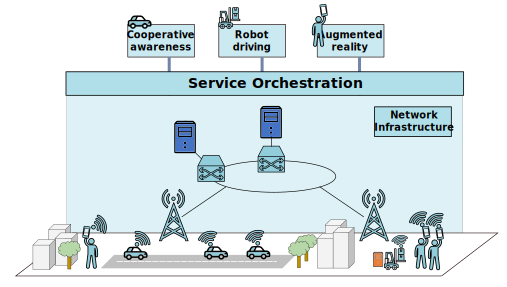
\includegraphics[width=\textwidth]{img/big-picture-infra-gen.pdf}
                \caption{Network infrastructure for service providing.}
                \label{fig:big-infra}
            \end{figure}
        \end{minipage}
    }
\end{frame}





\begin{frame}
    \frametitle{\secname}
    \framesubtitle{\subsecname}
    %
    \textbf{Location of BSs}:
    \begin{itemize}
        \item Neyman-Scott Poisson Cluster Process~\cite{vinay-moller-interference}
        \item Poisson Point Processes (PPPs)~\cite{stochastic-martina}
            \begin{itemize}
                \item homogeneous~\cite{cran-vinay-moller,hetnets-cor}
                \item hard-core~\cite{hard-core-cover} \pause
                \item {\color{red}\textbf{inhomogeneous \& Matérn~II}}
            \end{itemize}
    \end{itemize}
    \pause
    \vfill
    \hrule
    \vfill
    \textbf{Location of MEC PoPs}:
    \begin{itemize}
        \item along highways~\cite{usa-mec}
        \item within stadiums~\cite{tokio-olympics} \pause
        \item {\color{red}\textbf{population census}}
        \item {\color{red}\textbf{access \& aggregation rings}}
    \end{itemize}

\end{frame}


\subsection{Thesis contribution}
\begin{frame}
    \frametitle{Outline}
    \tableofcontents[subsectionstyle=show/shaded/hide,sectionstyle=show/shaded]
\end{frame}



\begin{frame}
    \frametitle{\secname}
    \framesubtitle{\subsecname}
    \vfill
    \begin{minipage}{0.27\textwidth}
        Derive:
        \begin{itemize}
            \item BS location
            \item MEC PoP server location
        \end{itemize}
        Meet:
        \begin{itemize}
            \item Tactile RTT of \mbox{\textbf{1 ms}}
        \end{itemize}
    \end{minipage}
    \hfill
    \begin{minipage}{0.68\textwidth}
        \begin{figure}
            \centering
            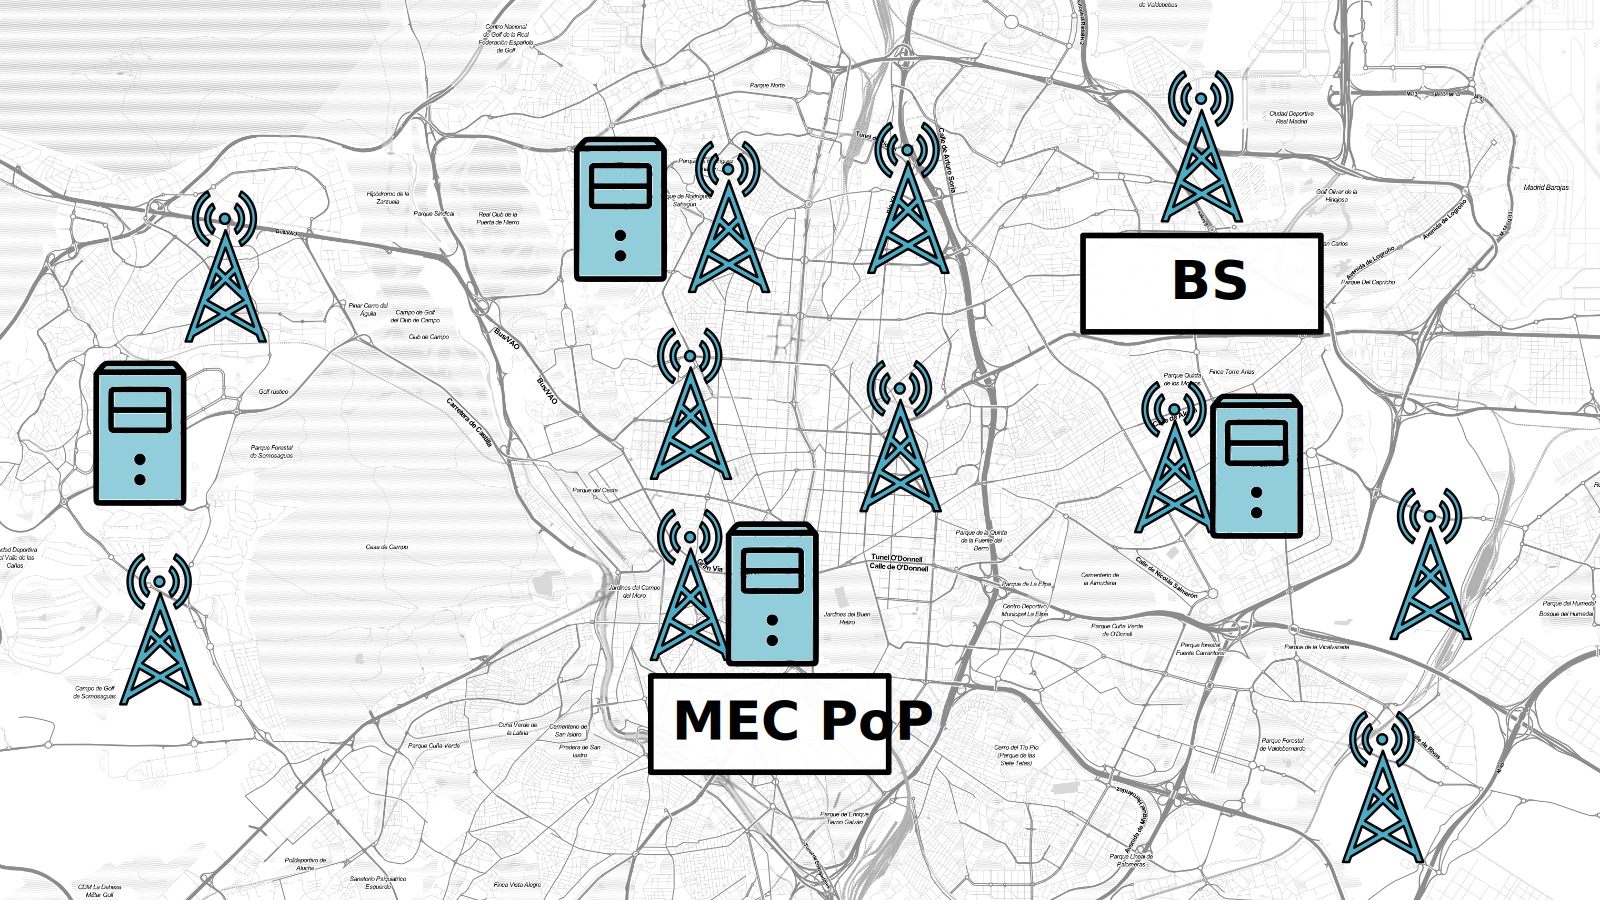
\includegraphics[width=\textwidth]{img/pop-and-antennas.pdf}
            \caption{BS and MEC PoP locations.}
            \label{fig:bs-pop-locations}
        \end{figure}
    \end{minipage}
    \vfill
\end{frame}




\begin{frame}
    \frametitle{\secname}
    \framesubtitle{\subsecname}

    Higher gentrification $\implies$ more BSs
    \vfill

    \begin{minipage}{.35\textwidth}
        \begin{itemize}
            \item $R$ -- region of interest
            \item $C_i$ -- area
            \onslide<2->{\item $f_i(x)$ -- revolution func.}
            \onslide<3->{\item $G(x)$ -- gentrification \\ \begin{itemize} \item $G(x)=\sum_i f_i(x)$\end{itemize}}
        \end{itemize}
    \end{minipage}
    \begin{minipage}{.64\textwidth}
        \begin{figure}
            \centering
            \begin{tikzpicture}
                \node[inner sep=0pt] (russell) at (0,0) {
                    \only<1>{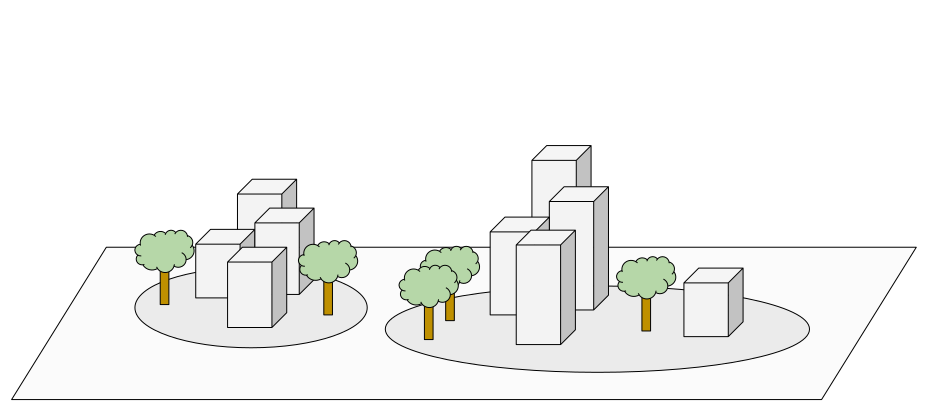
\includegraphics[width=\textwidth]{img/revolution-function-areas.pdf}}%
                    \only<2>{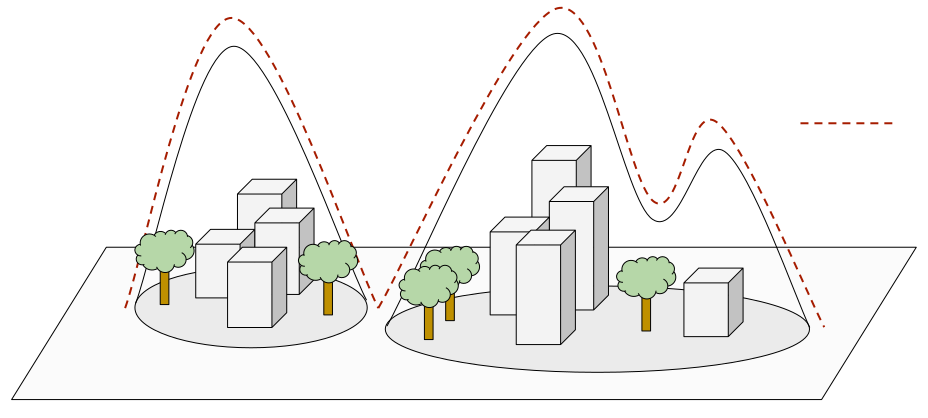
\includegraphics[width=\textwidth]{img/revolution-function-fs.pdf}}%
                    \only<3>{\includegraphics[width=\textwidth]{img/revolution-function.pdf}}
                };
                % \node[inner sep=0pt] (russell) at (0,0) {\includegraphics[width=\textwidth]{img/revolution-function}};
                \node at (-2.6,-1.5) {$C_1$};
                \node at (-.4,-1.6) {$C_2$};
                \node at (-4,-1.65) {$R$};
                \onslide<2->{\node at (-2.2,1) {$f_1$};}
                \onslide<2->{\node at (.9,1.2) {$f_2$};}
                \onslide<3->{\node at (3.6, 1.2) {$G(x)$};}
            \end{tikzpicture}
            \caption{\emph{Revolution functions} of a region with two building areas.}
            \label{fig:rev}
        \end{figure}
    \end{minipage}

\end{frame}





\begin{frame}
    \frametitle{\secname}
    \framesubtitle{\subsecname}

    \onslide<1-2>{\!\!}
    \onslide<3->{$\lambda(x)\sim G(x)$ probability of BS at $x$.}

    \vfill

    \begin{figure}
        \centering
        \only<1>{\includegraphics[width=.8\textwidth]{img/grid-left.pdf}}%
        \only<2>{\includegraphics[width=.8\textwidth]{img/grid-zoom.pdf}}%
        \only<3>{\includegraphics[width=.8\textwidth]{img/grid-points.pdf}}%
        \only<4>{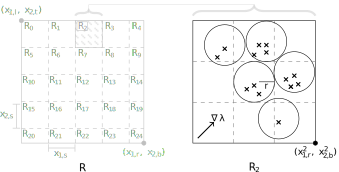
\includegraphics[width=.8\textwidth]{img/grid-radius.pdf}}%
        \only<5>{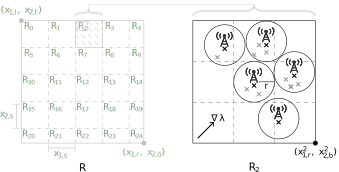
\includegraphics[width=.8\textwidth]{img/grid-final-antennas.pdf}}
        %% \begin{tikzpicture}[scale=.65,every node/.style={scale=0.65}]
    %%%%%%%%%%%%%%%%%%%%%
    % Gridded rectangle %
    %%%%%%%%%%%%%%%%%%%%%
    % Top brace
    \draw [ultra thick, decorate,decoration={brace,amplitude=4pt}] (2.2,5.2) -- (3.3,5.2) node [black,midway,yshift=0.5cm] {};

    \draw (0,0) rectangle (5,5);
    \foreach \c in {1.1, 2.2, 3.3, 4.4} {
        \draw[dashed, color=gray] (\c, 0) -- (\c, 5);
    }
    \foreach \r in {3.9, 2.8, 1.7, 0.6} {
        \draw[dashed, color=gray] (0, \r) -- (5, \r);
    }


    % Area names
    \edef\index{0}
    \foreach \r in {5, 3.9, 2.8, 1.7, 0.6} {
        \foreach \c in {0, 1.1, 2.2, 3.3, 4.4} {
            \node at (\c + 0.3, \r - 0.25) {\small{$R_{\index}$}};
            \pgfmathparse{int(\index+1)}
            \xdef\index{\pgfmathresult}
        }
    }

    % hashed area
    \draw[fill=white] (2.2,5) rectangle (3.3,3.9);
    \draw[pattern=north west lines, pattern color=black] (2.2,5) rectangle (3.3,3.9);
    \draw[fill=white] (2.27, 4.95) rectangle (2.7, 4.6);
    \node[name=highlighted] at (2.5, 4.75){\small{$R_2$}};

    % Top left coordinate
    \draw[fill=black] (0,5) circle [radius=2.5pt];
    \node at (0, 5.4) {$(x_{1,l},\ x_{2,t})$};

    % Bottom right coordinate
    \draw[fill=black] (5,0) circle [radius=2.5pt];
    \node at (5, -0.4) {$(x_{1,r},\ x_{2,b})$};

    % x1 side
    \draw[|-|] (1.1, -0.2) -- (2.2, -0.2);
    \node at (1.6, -0.5) {$x_{1,s}$};

    % x2 side
    \draw[|-|] (-0.2, 0.6) -- (-0.2, 1.6);
    \node at (-0.6, 1.1) {$x_{2,s}$};

    % Region tag
    \node at (2.5, -1) {\large{$R$}};


    %%%%%%%%%%%%%%%%%%
    % AAUs Matern II %
    %%%%%%%%%%%%%%%%%%
    \draw (2.75,5.3) -- (2.75, 5.65) -- (9.5, 5.65) -- (9.5, 5.5);
    % Top brace
    \draw [ultra thick, decorate,decoration={brace,amplitude=7pt}] (7,5.2) -- (12,5.2) node [black,midway,yshift=0.5cm] {};

    % Region tag
    \node at (9.5, -1) {\large{$R_2$}};


    % Bottom right coordinate
    \draw[fill=black] (12,0) circle [radius=2.5pt];
    \node at (12, -0.4) {$(x_{1,r}^2,\ x_{2,b}^2)$};

    \draw (7,0) rectangle (12,5);
    \foreach \r in {1.66, 3.32} {
        \draw[dashed, color=gray] (7, \r) -- (12, \r);
    }
    \foreach \c in {8.66, 10.32} {
        \draw[dashed, color=gray] (\c, 0) -- (\c, 5);
    }

    % Center AAU
    \draw[color=gray] (9.7, 2.5) -- (10.32, 2.5);
    \node[cross out, draw, anchor=text, thick, color=gray, line cap=round, scale=0.5] at (9.5, 2.35) {};
    \node at (9.5, 2.5) {\includegraphics[width=0.02\textwidth]{img/base-station}};
    \draw[color=gray] (9.5, 2.5) circle (0.83);
    \node at (10, 2.3) {\small{$r$}};
    % Non-survival AAU
    \node[cross out, draw, anchor=text, thick, color=gray, line cap=round, scale=0.5] at (9.2, 2.2) {};
    \node[cross out, draw, anchor=text, thick, color=gray, line cap=round, scale=0.5] at (9.7, 2) {};
    
    % Bottom right AAU
    \node[cross out, draw, anchor=text, thick, color=gray, line cap=round, scale=0.5] at (10.5, 0.85) {};
    \node at (10.5, 1) {\includegraphics[width=0.02\textwidth]{img/base-station}};
    \draw[color=gray] (10.5, 1) circle (0.83);
    %\node[cross out, draw, anchor=text, thick, color=gray, line cap=round, scale=0.5] at (10.7, 0.4) {};
    %\node[cross out, draw, anchor=text, thick, color=gray, line cap=round, scale=0.5] at (10,1.2) {};
    %\node[cross out, draw, anchor=text, thick, color=gray, line cap=round, scale=0.5] at (10.2, 0.8) {};

    % Center right AAU
    \node[cross out, draw, anchor=text, thick, color=gray, line cap=round, scale=0.5] at (11.14, 2.75) {};
    \node at (11.14, 2.9) {\includegraphics[width=0.02\textwidth]{img/base-station}};
    \draw[color=gray] (11.14, 2.9) circle (0.83);
    \node[cross out, draw, anchor=text, thick, color=gray, line cap=round, scale=0.5] at (11.3, 2.4) {};
    \node[cross out, draw, anchor=text, thick, color=gray, line cap=round, scale=0.5] at (10.8, 2.6) {};
    \node[cross out, draw, anchor=text, thick, color=gray, line cap=round, scale=0.5] at (11, 2.3) {};

    % Top AAU
    \node[cross out, draw, anchor=text, thick, color=gray, line cap=round, scale=0.5] at (10, 4) {};
    \node at (10, 4.15) {\includegraphics[width=0.02\textwidth]{img/base-station}};
    \draw[color=gray] (10, 4.15) circle (0.83);
    \node[cross out, draw, anchor=text, thick, color=gray, line cap=round, scale=0.5] at (11, 2.3) {};
    \node[cross out, draw, anchor=text, thick, color=gray, line cap=round, scale=0.5] at (9.7, 4) {};
    \node[cross out, draw, anchor=text, thick, color=gray, line cap=round, scale=0.5] at (10, 3.7) {};
    \node[cross out, draw, anchor=text, thick, color=gray, line cap=round, scale=0.5] at (9.5, 3.6) {};

    % Top left AAU
    \node[cross out, draw, anchor=text, thick, color=gray, line cap=round, scale=0.5] at (8.3, 3.85) {};
    \node at (8.3, 4) {\includegraphics[width=0.02\textwidth]{img/base-station}};
    \draw[color=gray] (8.3, 4) circle (0.83);
    \node[cross out, draw, anchor=text, thick, color=gray, line cap=round, scale=0.5] at (8,3.5) {};

    % lambda increasing direction
    \draw[thick, ->] (7.2, 0.2) -- (7.86, 0.86) node[pos=1.25]{$\nabla\lambda$};

\end{tikzpicture}

        \caption{Inhomogeneous Mattérn~II process.}
        \label{fig:grid-aau-gen}
    \end{figure}
\end{frame}



% \begin{frame}
%     \frametitle{\secname}
%     \framesubtitle{\subsecname}
% 
%     \begin{minipage}{.48\textwidth}
%         \begin{itemize}
%             \item $G(x)$: Madrid census
%             \item $R$: Madrid city
%             \item Inhomogeneous Mattern~II PPs
%         \end{itemize}
%     \end{minipage}
%     \begin{minipage}{.5\textwidth}
%         \begin{figure}
%             \centering
%             \includegraphics[width=.9\textwidth]{img/madrid-map-antennas.png}
%             \caption{Location of BSs}
%             \label{fig:bs-location}
%         \end{figure}
%     \end{minipage}
% \end{frame}





\begin{frame}
    \frametitle{\secname}
    \framesubtitle{\subsecname}

    \begin{minipage}{.48\textwidth}
        \only<2>{\color{gray}}
        Inhomogeneous Mattérn~II PPs applied on:
        \begin{itemize}
            \item \only<2>{\color{gray}} $R$: Madrid city
            \item \only<2>{\color{gray}} $G(x)$: Madrid census
        \end{itemize}
    \end{minipage}
    \begin{minipage}{.5\textwidth}
        \begin{figure}
            \centering
            \only<1>{\includegraphics[width=.9\textwidth]{img/madrid-map-antennas.png}}%
            \only<2>{\includegraphics[width=.9\textwidth]{img/where-pop.pdf}}
            \caption{Location of BSs.}
            \label{fig:bs-location}
        \end{figure}
    \end{minipage}
\end{frame}





\begin{frame}
    \frametitle{\secname}
    \framesubtitle{\subsecname}

    \begin{figure}
        \centering
        \only<1>{\includegraphics[width=1.0\textwidth]{img/infrastructure.pdf}}%
        \only<2>{\includegraphics[width=1.0\textwidth]{img/infrastructure-mec-pop-m1.pdf}}%
        \only<3>{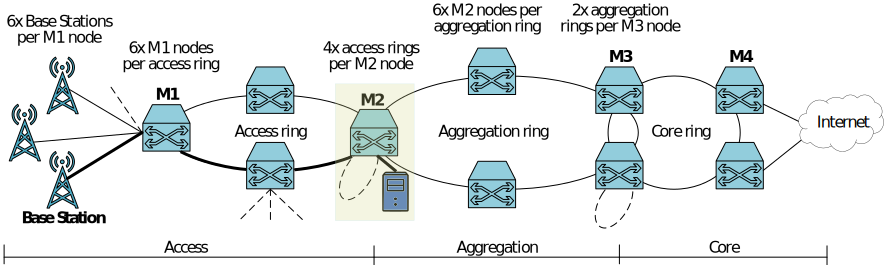
\includegraphics[width=1.0\textwidth]{img/infrastructure-mec-pop-m2.pdf}}%
        \caption{Reference network infrastructure as illustrated\footnote{Author: Dr. Luca Cominardi.} in~\cite{8436847} and based on~\cite{itu.t.ref.arch}. }
        \label{fig:infrastructure}
    \end{figure}
\end{frame}





\begin{frame}
    \frametitle{\secname}
    \framesubtitle{\subsecname}

    Derive MEC PoP location considering:


    \begin{equation}
        \only<1>{RTT = 2d\cdot5\frac{\mu s}{km} + 2M\cdot 50\mu s + UL + DL}
        \only<2>{RTT = \highlight{2d\cdot5\frac{\mu s}{km}}{fiber propagation} + 2M\cdot 50\mu s + UL + DL}
        \only<3>{RTT = 2d\cdot5\frac{\mu s}{km} + \highlight{2M\cdot 50\mu s}{ring propagation} + UL + DL}
        \only<4>{RTT = 2d\cdot5\frac{\mu s}{km} + 2M\cdot 50\mu s + \highlight{UL + DL}{radio propagation}}
        \label{eq:rtt-bad}
    \end{equation}

    \vfill

    \begin{itemize}
        \item $d$: distance between BS and MEC PoP
        \item $M$: \#traversed rings (e.g., $1,2,\ldots$)
        \item $UL$: Uplink propagation latency
        \item $DL$: Downlink propagation latency
    \end{itemize}

\end{frame}





\begin{frame}
    \frametitle{\secname}
    \framesubtitle{\subsecname}

    \centering{
        \only<1>{$m_M$: maximum distance between MEC PoP at ring $M$ and BS}
        \only<2>{$m_2$: maximum distance between MEC PoP at ring $2$ and BS}
    }
    \begin{figure}
        \centering
        \only<1>{\includegraphics[width=0.7\textwidth]{img/generation-algo-1.pdf}}%
        \only<2>{\includegraphics[width=0.7\textwidth]{img/generation-algo-2.pdf}}
        \caption{How to select MEC PoP location.}
        \label{fig:algo-pop-location}
    \end{figure}
\end{frame}






\begin{frame}
    \frametitle{\secname}
    \framesubtitle{\subsecname}


\begin{figure}
    \centering
    % \comment{!!! @Jorge: this is still here!!! We need to improve the figures captions. It's hard to understand what the figures show only by looking at the pictures. It is not explained in the what $C_{A,M2}$ means. !!!}
    \subfigure[FDD 120 kHz 7s]{ \includegraphics[clip, trim=0cm 2.7cm 0.25cm 3cm, width=0.35\textwidth]{img/madrid-ii-m2.png}}
        ~
    \subfigure[TDD 120 kHz 7s]{\includegraphics[clip, trim=0cm 2.7cm 0.25cm 3cm, width=0.35\textwidth]{img/madrid-i-iii-m2.png}}\\
    \caption{\textbf{Urban scenario} (Madrid city center) -- $C_{A,M2}=$covered BSs.}
    \label{fig:madrid}
\end{figure}

\end{frame}





\begin{frame}

    \frametitle{\secname}
    \framesubtitle{\subsecname}

\begin{figure}
    \centering
    \subfigure[FDD 120 kHz 7s]{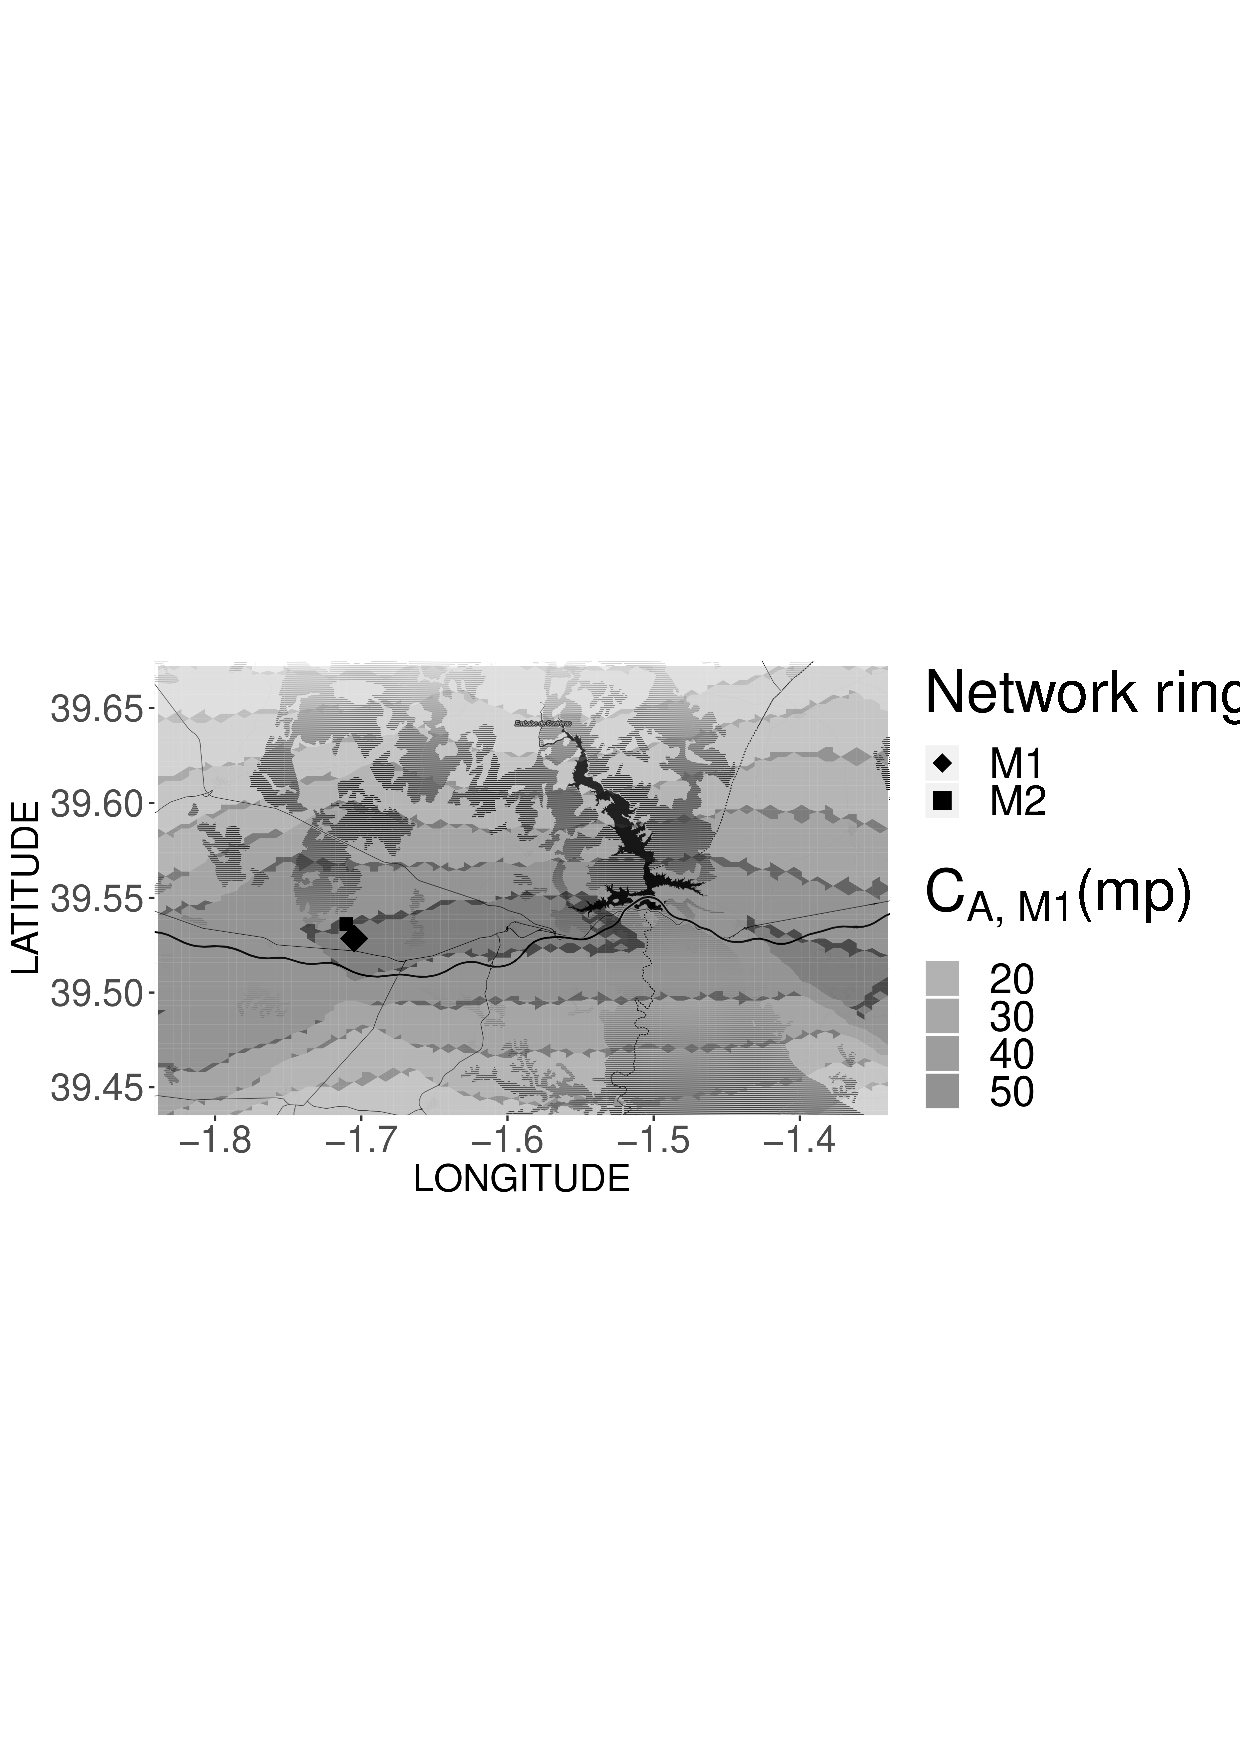
\includegraphics[clip, trim=0cm 8.5cm 0.25cm 6.7cm, width=0.485\textwidth]{img/hoces-del-cabriel-ii-m1.png}}
     ~                       
    \subfigure[TDD 120 kHz 7s]{\includegraphics[clip, trim=0cm 8.5cm 0.25cm 6.7cm, width=0.485\textwidth]{img/hoces-del-cabriel-i-iii-m1.png}}\\
    \caption{\textbf{Highway scenario} (Hoces del Cabriel A3) -- $C_{A,M1}=$covered BSs by M1 MEC PoP.}
    \label{fig:madrid}
\end{figure}

\end{frame}





\begin{frame}

    \frametitle{\secname}
    \framesubtitle{\subsecname}

    \begin{figure}[t]
        \centering
        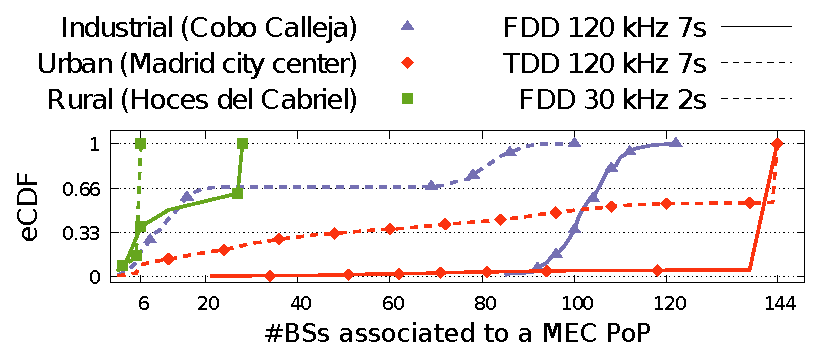
\includegraphics[width=.8\columnwidth]{img/cdfs}
        \vspace{1em}
        \caption{eCDF of the number of BSs assigned to a MEC PoP in the studied scenarios.}
        % \comment{LC: Increase the axis and label font size}
        \label{fig:cdfs}
    \end{figure}
\end{frame}


\subsection{Output}
\begin{frame}
    \frametitle{Outline}
    \tableofcontents[subsectionstyle=show/shaded/hide,sectionstyle=show/shaded]
\end{frame}

\begin{frame}
    \frametitle{\secname}
    \framesubtitle{\subsecname}
    Publications:
    \begin{itemize}
        \item \fullcite{modelling-bs}
        \item \fullcite{5gen}
    \end{itemize}
    Open-source:
    \begin{itemize}
        \item \textbf{BS \& MEC PoP generation}: \url{github.com/MartinPJorge/mec-generator/}
        \item \textbf{5GEN}: \url{https://github.com/MartinPJorge/mec-generator/tree/5g-infra-gen/}
    \end{itemize}
    

\end{frame}






\section{NFV Orchestration in federated environments}
\subsection{State of the art}
\begin{frame}
    \frametitle{Outline}
    \tableofcontents[subsectionstyle=show/shaded/hide,sectionstyle=show/shaded]
\end{frame}





\begin{frame}
    \frametitle{\secname}
    \framesubtitle{\subsecname}

    \begin{figure}
        \centering
        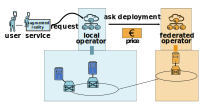
\includegraphics[width=\textwidth]{img/federation.pdf}
        \caption{Service federation.}
        \label{fig:federation}
    \end{figure}

\end{frame}





\begin{frame}
    \frametitle{\secname}
    \framesubtitle{\subsecname}


    % Horizon2020 projects dealing with federation:
    % \begin{itemize}
    %     \item 5GEx~\cite{5gex-prototype}, 5G-TRANSFORMER~\cite{5g-transformer}, 5GROWTH~\cite{5growth}
    % \end{itemize}\pause

    Orchestration and \textbf{fixed pricing} in multi-domain:
    \begin{itemize}
        \item Alternating Direction Method of Multipliers (ADMM)~\cite{ad3Distributed}
        \item branching heuristic~\cite{consolidation}
        \item graph-based message passing~\cite{vertex-centric}
        \item greedy with backtracking~\cite{balazsEmbedding} \pause
        \item \textbf{\color{red}cutoffs in Dijkstra, DFS and BFS~\cite{multi-domain-msc}}
        \item \textbf{\color{red}Q-learning federation~\cite{icc}}
    \end{itemize} \pause
    Orchestration and \textbf{\color{red}dynamic pricing} in multi-domain: \pause
    \begin{itemize}
        \item \textbf{\color{red}real-price traces AWS}\pause
        \item \textbf{\color{red}Deep Q-learning}\pause
        \item \textbf{\color{red}Telefónica scenario}
    \end{itemize}
\end{frame}



\subsection{Thesis contribution}
\begin{frame}
    \frametitle{Outline}
    \tableofcontents[subsectionstyle=show/shaded/hide,sectionstyle=show/shaded]
\end{frame}


\begin{frame}
    \frametitle{\secname}
    \framesubtitle{\subsecname}

    \begin{figure}
        \centering
        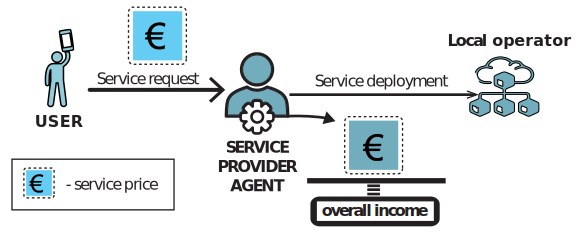
\includegraphics[width=.8\textwidth]{img/local-deploy.pdf}
        \caption{Business model - local deployment\footnote{Based on Kiril Antevski illustration}.}
        \label{fig:local-deploy}
    \end{figure}
\end{frame}



\begin{frame}
    \frametitle{\secname}
    \framesubtitle{\subsecname}

    \begin{figure}
        \centering
        \only<1>{\includegraphics[width=.7\textwidth]{img/federation-deploy.pdf}}%
        \only<2>{\includegraphics[width=.7\textwidth]{img/federation-deploy-we-are.pdf}}%
        \only<3>{\includegraphics[width=.7\textwidth]{img/federation-deploy-changes.pdf}}%
        \only<4>{\includegraphics[width=.7\textwidth]{img/federation-deploy-they-change.pdf}}%
        \caption{Business model - federate deployment\footnote{Based on Kiril Antevski illustration}.}
        \label{fig:fed-deploy}
    \end{figure}
\end{frame}



\begin{frame}
    \frametitle{\secname}
    \framesubtitle{\subsecname}
    \begin{minipage}{0.3\textwidth}
        \textit{t3a.small}:
        \begin{itemize}
            \item 2 CPUs
            \item memory 2 GB
            \item storage 100 GB
        \end{itemize}
    \end{minipage}
    \begin{minipage}{0.65\textwidth}
        \begin{figure}
            \centering
            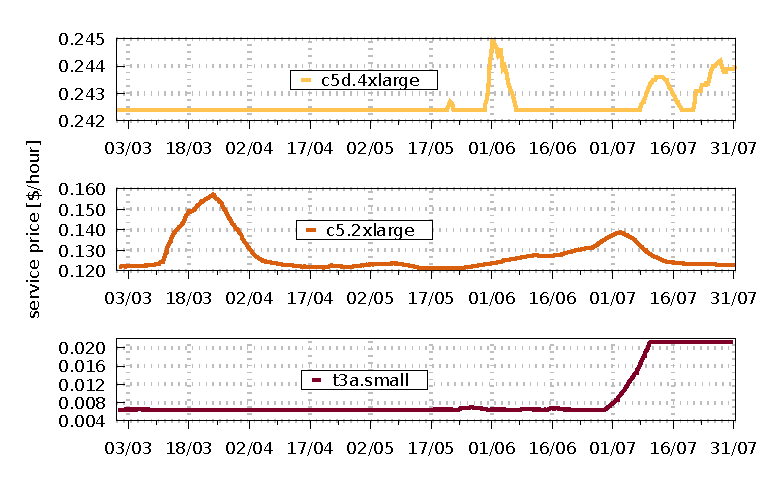
\includegraphics[width=\textwidth]{img/experiment-aws-prices}
            \caption{AWS service prices during 2020 in west Europe.}
            \label{fig:aws-prices}
        \end{figure}
    \end{minipage}
\end{frame}


\begin{frame}
    \frametitle{\secname}
    \framesubtitle{\subsecname}

    \begin{figure}
        \centering
        \includegraphics[width=.65\textwidth]{img/rho-arrivals}
        \caption{Impact of prices on arriving users -- based on tid study~\cite{tid} and~\cite{xavierPricing}.}
        \label{fig:arrivals}
    \end{figure}
\end{frame}


\begin{frame}
    \frametitle{\secname}
    \framesubtitle{\subsecname}

    \begin{minipage}{.4\textwidth}
        Considering:
        \begin{itemize}
            \item Price changes
            \item Available resources (CPU, memory, disk)
            \item Service lifetime (e.g., 2 days)
        \end{itemize}
        \only<1>{\vspace{6em}}
        \only<2>{For each service $\sigma$, decide / take an \textbf{action}:
            \begin{itemize}
                \item $x(\sigma)=0$: \textbf{reject} 
                \item $x(\sigma)=1$: \textbf{local} 
                \item $x(\sigma)=2$: \textbf{federate}
            \end{itemize}
        }
    \end{minipage}
    \begin{minipage}{.5\textwidth}
        \only<2>{\begin{figure}
                \centering
                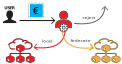
\includegraphics[width=.8\textwidth]{img/decisions}
                \caption{Possible actions.}
                \label{fig:decisions}
            \end{figure}
        }
    \end{minipage}
\end{frame}





\begin{frame}
    \frametitle{\secname}
    \framesubtitle{\subsecname}


    \begin{minipage}{.45\textwidth}
        Obtained \textbf{reward}:
        \begin{multline}
            \only<1>{r^{(t)}(X_t) := \sum_{\substack{\sigma:~ x(\sigma)=0\\a(\sigma) \le t\le d(\sigma)}}p^{a(\sigma)}(\sigma) + \\
            \sum_{\substack{\sigma:~ x(\sigma)=1\\ a(\sigma) \le t\le d(\sigma)}} \left[ p^{a(\sigma)}(\sigma) - f^{(t)}(\sigma) \right]}
            \only<2>{r^{(t)}(X_t) := \highlight[upper={fill=red!20},lower={fill=red!20},line={red!20}]{\sum_{\substack{\sigma:~ x(\sigma)=0\\a(\sigma) \le t\le d(\sigma)}}p^{a(\sigma)}(\sigma)}{local} + \\
            \sum_{\substack{\sigma:~ x(\sigma)=1\\ a(\sigma) \le t\le d(\sigma)}} \left[ p^{a(\sigma)}(\sigma) - f^{(t)}(\sigma) \right]}
            \only<3>{r^{(t)}(X_t) := \sum_{\substack{\sigma:~ x(\sigma)=0\\a(\sigma) \le t\le d(\sigma)}}p^{a(\sigma)}(\sigma) + \\
            \highlight[upper={fill=yellow!20},lower={fill=yellow!20},line={yellow!20}]{\sum_{\substack{\sigma:~ x(\sigma)=1\\ a(\sigma) \le t\le d(\sigma)}} \left[ p^{a(\sigma)}(\sigma) - f^{(t)}(\sigma) \right]}{federation}}
            \label{eq:instant-reward-highlighted}
        \end{multline}

    \end{minipage}
    \begin{minipage}{.5\textwidth}
    \begin{figure}
        \centering
        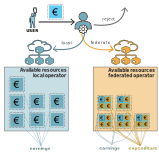
\includegraphics[width=.9\textwidth]{img/available}
        \caption{Environment snapshot at time $t$.}
        \label{fig:earnings-actions}
    \end{figure}
    \end{minipage}
\end{frame}




\begin{frame}
    \frametitle{\secname}
    \framesubtitle{\subsecname}


    \begin{minipage}{.45\textwidth}
        \textbf{Online optimization problem}:
        \begin{itemize}
            \item objective: $\max_{X_t} \frac{1}{T}\sum_t r^{(t)}(X_t)$
            \item constraints:
                \begin{itemize}
                    \item CPU
                    \item memory
                    \item disk
                \end{itemize}
        \end{itemize}
        NP-hard: knapsack problem equivalence
    \end{minipage}\pause
    \hfill
    \vline
    \hfill
    \begin{minipage}{.45\textwidth}
        \textbf{Markov Decision Problem} (MDP):
        \begin{itemize}
            \item find policy $\pi$ to: $\max_\pi \mathbb{E}_{x(\sigma)\sim\pi}\left[ \sum_t \gamma^{t}\ r^{(t)}(\pi) \right]$
            \item action space $\mathcal{A}=\{0,1,2\}$
            \item state space $\mathcal{S}$:
                \begin{itemize}
                    \item available \& requested resources
                    \item current prices
                    \item service lifetime
                \end{itemize}
            \item instant reward $r^{(t)}(\pi)$
        \end{itemize}
    \end{minipage}
    
\end{frame}







\begin{frame}
    \frametitle{\secname}
    \framesubtitle{\subsecname}

    \begin{figure}
        \centering
        % MLP 2 hidden layers


\begin{tikzpicture}[scale=.65,every node/.style={scale=0.65}]
    \input{network_init}
    
    
    
    \def\nodedist{35pt}
    \def\layerdist{2}
    \def\pindist{20pt}
    
    \tikzstyle{every pin edge}=[signal]
    \tikzstyle{annot} = [text width=4em, text centered]
    
    % define blocks top left corners
    %% state block %%
    \def\statex{4}
    \def\statey{0}
    %% epsilon block %%
    \def\epsilonx{4}
    \def\epsilony{2}
    %% 1-epsilon block %%
    \def\epsilonx{4}
    \def\epsilony{6}
    %% NN block %%
    \def\nnx{6}
    \def\nny{6}
    %% argmax block %%
    \def\argmaxx{14}
    \def\argmaxy{{\nny-0.5*\nodedist-\nodedist}}
    %% random block %%
    \def\randomx{\argmaxx}
    \def\randomy{\statey}
    %% max Q(a) block %%
    \def\maxqax{14}
    \def\maxqay{{\nny-0.5*\nodedist-2*\nodedist}}
    %% Q(a) block %%
    \def\qax{14}
    \def\qay{{\nny-0.5*\nodedist-3*\nodedist}}
    %% loss block %%
    \def\lossx{18}
    \def\lossy{\qay}
    %% ENV block %%
    \def\envx{20}
    \def\envy{0}
    %% experience block %%
    \def\experiencex{\envx}
    \def\experiencey{-6.5}
    %% adder block %%
    \def\addx{{\maxqax+3}}
    \def\addy{\maxqay}
    %% minus block %%
    \def\minusx{{\addx}}
    \def\minusy{\qay}
    
    %%%%%%%%%%%%%%%%%
    %% State block %%
    %%%%%%%%%%%%%%%%%
    \def\xx{\statex}
    \def\yy{\statey}
    \node (state) [] at (\xx, \yy) { $s^{(t)}$};
    
    
    %%%%%%%%%%%%%%%%%
    %% random block %%
    %%%%%%%%%%%%%%%%%
    \def\xx{\randomx}
    \def\yy{\randomy}
    \node (random) [rectangle,draw,anchor=west,fill=red!10] at (\xx,\yy) {Random action};
    
    %%%%%%%%%%%%%%%%%
    %% loss block %%
    %%%%%%%%%%%%%%%%%
    \def\xx{\lossx}
    \def\yy{\lossy}
    \node (loss) [rectangle,draw,anchor=west,fill=yellow!10] at (\xx,\yy) {$\nabla_{\vec{w}} L$};    
    
    %%%%%%%%%%%%%%%%%
    %% argmax block %%
    %%%%%%%%%%%%%%%%%
    \def\xx{\argmaxx}
    \def\yy{\argmaxy}
    \node (argmaxQ) [rectangle,draw,anchor=west,fill=red!10] at (\xx,\yy) {$\argmax_x Q(s,x)$};
    
    %%%%%%%%%%%%%%%%%
    %% max Q(a) block %%
    %%%%%%%%%%%%%%%%%
    \def\xx{\maxqax}
    \def\yy{\maxqay}
    \node (maxQ) [rectangle,draw,anchor=west,fill=yellow!10] at (\xx,\yy) {$\max_x Q(s,x)$};
    
    %%%%%%%%%%%%%%%%%
    %% Q(a) block %%%
    %%%%%%%%%%%%%%%%%
    \def\xx{\qax}
    \def\yy{\qay}
    \node (Qa) [rectangle,draw,anchor=west,fill=yellow!10] at (\xx,\yy) {$Q(x)$};
    
    %%%%%%%%%%%%%%%%%
    %% adder block %%%
    %%%%%%%%%%%%%%%%%
    \def\xx{\addx}
    \def\yy{\addy}
    \node (adder) [circle,inner sep=0.1,draw,anchor=west] at (\xx,\yy) {$+$};
    
    %%%%%%%%%%%%%%%%%
    %% minus block %%%
    %%%%%%%%%%%%%%%%%
    \def\xx{\minusx}
    \def\yy{\minusy}
    \node (minus) [circle,inner sep=0.1,draw,anchor=west] at (\xx,\yy) {$-$};
    
    
    %%%%%%%%%%%%%%%%%
    %% ENV block %%
    %%%%%%%%%%%%%%%%%
    \def\xx{\envx}
    \def\yy{\envy}
    \node (env) [rectangle,inner ysep=15pt,draw,anchor=center,fill=red!10] at (\xx,\yy) {Environment};
    \node (actiondot) [circle,fill=black,inner sep=2pt,label=right:$x$] at (\xx-1.8,\yy) {};
    
    
    %%%%%%%%%%%%%%%%%
    %% experience block %%
    %%%%%%%%%%%%%%%%%
    \def\xx{\experiencex}
    \def\yy{\experiencey}
    \node (experience) [rectangle,inner ysep=8pt,draw,anchor=center,fill=yellow!10] at (\xx,\yy) {Experience};
    
    
    %%%%%%%%%%%%%%
    %% NN BLOCK %%
    %%%%%%%%%%%%%%
    % set reference point to the NN block
    \def\xx{\nnx}
    \def\yy{\nny}
    
    \node (indot) [circle,fill=black,inner sep=2pt,label=right:$s$] at (\xx-1,\yy-2.5*\nodedist) {};

    % Input layer neurons
    \foreach \y in {1,...,4}
        \node[inputnode] 
            (I\y) at (\xx,\yy-\y*\nodedist) {$b_{\y}$};  

    % Hidden layer neurons
    \foreach \y in {1,...,4}
        \node[hiddennode] 
            (H\y) at 
            (\xx+\layerdist,\yy-\y*\nodedist) {$z_{\y}$};
            %($(\xx+\layerdist,\yy-\y*\nodedist) +(0, 0.5*\nodedist)$) {$z_{\y}$};
    
    % Output layer
    \foreach \y in {0,...,2}
        \node[outputnode, pin={[pin edge={-latex}, pin distance=\pindist]right:$Q(s,\y)$}]
            (O\y) at (\xx+2*\layerdist, {\yy-0.5*\nodedist-(\y+1)*\nodedist}) {$y_{\y}$};

    \foreach \dest in {1,...,4}
        \foreach \source in {1,...,4}
            \ifthenelse{\source=4}{\draw[signal, loosely dotted,color=gray] (I\source) -- (H\dest);}{\draw[signal] (I\source) -- (H\dest);};

    
    \foreach \dest in {0,...,2}
        \foreach \source in {1,...,4}
            \draw[signal] (H\source) edge (O\dest);
            
    % Brace
        \draw [decorate,decoration={brace,amplitude=10pt,raise=4pt},xshift=0pt] ($(O0)+(2.5,0)$) -- ($(O2)+(2.5,0)$) node (braceOut) [black,midway,right, xshift=0.2cm] {};
            
    %\node[annot, above=4pt of H11] (hl) {Hidden layer 1};
    %\node[annot] at (I1 |- hl) {Input layer};
    %\node[annot] at (O1 |- hl) {Output layer};
    %%%%%%%%%%%%%%%%%%
    %% end NN BLOCK %%
    %%%%%%%%%%%%%%%%%%
    
    
    %%%%%%%%%%%%%%%%%%%%
    %% TRAINING FLOWS %%
    %%%%%%%%%%%%%%%%%%%%
    \coordinate[left = 0.15cm of argmaxQ] (argmaxQL);
    \coordinate[left = 0.15cm of Qa] (QaL);
    \draw[->] (braceOut) -- (argmaxQL) ;
    \draw[dashdotted,->] (braceOut) -- (maxQ) ;
    \draw[dashdotted,->] (maxQ) -- (adder);
    \draw[dashed,->] (braceOut) -- (QaL) ;
    \draw[dashed,->] (Qa) -- (minus);
    \draw[dashdotted,->] (adder) -- (minus);
    \draw[dotted,->] (minus) -- (loss);
    \draw[loosely dotted,->] (loss) -- ($(loss) - (0,1.3)$) -- node[pos=0.7,fill=white] {$\delta\vec{w}$} ($(loss)-(0,1.3)-(11.5,0)$) -- ($(loss)-(0,0.8)-(11.5,0)$);
    % experience replay BUS
    \draw[dotted,->] (experience) -- node (sarsa) [pos=0.15,fill=white] {$\left\{ (s^{(\tau)}, x(\sigma_\tau), r^{(\tau)}, s^{(\tau+1)})\right\}_\tau$} ($(\nnx,\experiencey)-(2,0)$)  node (stau)[circle,fill=gray!30,inner sep=2] at ({\xx-1,\experiencey}) {} node (stau1)[circle,fill=gray!30,pos=1,inner sep=2]{} node (atau) [circle,fill=gray!30,inner sep=2] at ($(Qa) - (0,2.4)$){};
    \draw[dashdotted,->] let \p1 = (sarsa), \p2 = (loss), \p3 = (adder) in (\x1-60,\y1) -- node[circle,fill=gray!30,pos=0,inner sep=2]{} (\x1-60,\y1+20) -- (\x3+60,\y1+20) -- node[pos=0.3,fill=white] {$r^{(\tau)}$} (\x3+60,\y3) -- (adder);
    % experience replay input
    \draw[dashed,->] (atau) -- (Qa) node [pos=0.7,fill=white] {$x(\sigma_\tau)$};
    \draw[dashed,->] (stau) -- (indot) node [pos=0.3,fill=white] {$s^{(\tau)}$};
    \draw[dashed,->] (stau) -- (indot) node [pos=0.3,fill=white] {$s^{(\tau)}$};
    \draw[dashdotted,->] let \p1 = (indot),\p2 = (stau1) in (stau1) -- node [pos=0.5,fill=white] {$s^{(\tau+1)}$} (\x2,\y1) -- (indot);
    
    %%%%%%%%%%%%%%%%%%%%%
    %% EXECUTION FLOWS %%
    %%%%%%%%%%%%%%%%%%%%%
    \draw[->,fill=black] let \p1 = (indot) in (state) -- (random) node (epsilon) [circle,fill=gray,inner sep=2] at (\x1,\statey) {} node [pos=0.5,fill=white] {$\epsilon$};
    \draw[->] (epsilon) -- node [pos=0.2,fill=white] {$1-\epsilon$} (indot);
    \draw[->] (random) -- (actiondot); 
    \draw[->] let \p1 = (actiondot), \p2 = (argmaxQ) in (argmaxQ) -- (\x1,\y2) -- (actiondot); 
    \draw[->]  (\envx,\envy+0.8) -- (\envx,{\envy+1}) -- node [pos=0.05,fill=white] {$s^{(t+1)}$} (\statex,\statey+1) -- (state); 
    \draw[->] (\envx+1,\envy) -- (\envx+1.5,\envy) node [right] {$r^{(t)}$};
    \draw[dotted,->] (env) -- node [pos=0.3,fill=white] {$(s^{(t)}, x(\sigma_t), r^{(t)}, s^{(t+1)})$} (experience);
    

\end{tikzpicture}

        \caption{DQN architecture to decide rejection/local/federate.}
    \end{figure}
\end{frame}



\begin{frame}
    \frametitle{\secname}
    \framesubtitle{\subsecname}

    \textbf{Experimentation}:
    \begin{itemize}
        \item Telefónica infrastructure \& resources~\cite{tid}\pause
        \item AWS prices dataset:
            \begin{itemize}
                \item training 29/02/2020 -- 02/05/2020
                \item testing\! 03/05/2020 --31/07/2020
            \end{itemize}\pause
        \item Poissonian arrival of users
    \end{itemize}
\end{frame}





\begin{frame}
    \frametitle{\secname}
    \framesubtitle{\subsecname}

    \begin{minipage}{0.27\textwidth}
        Comparison of:
        \begin{itemize}
            \item Optimal
            \item DQN
            \item Q-table
            \item Q-table explore
            \item greedy
        \end{itemize}
        \only<3->{Results:
            \begin{itemize}
                \item near-optimal
                \only<5>{\item react upon peaks}
            \end{itemize}
        }
    \end{minipage}
    \begin{minipage}{0.65\textwidth}
    \begin{figure}
        \centering
        
        \only<1>{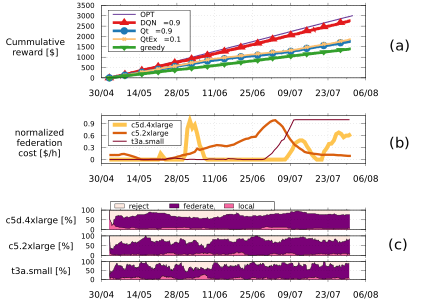
\includegraphics[width=\textwidth]{img/cdfs-all-decisions_edited_dqn.pdf}}%
        \only<2>{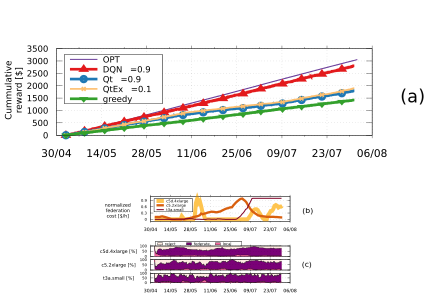
\includegraphics[width=\textwidth]{img/cdfs-all-decisions_edited_dqn-zoom-cdf.pdf}}%
        \only<3>{\includegraphics[width=\textwidth]{img/cdfs-all-decisions_edited_dqn-zoom-cdf-highlighter.pdf}}%
        \only<4>{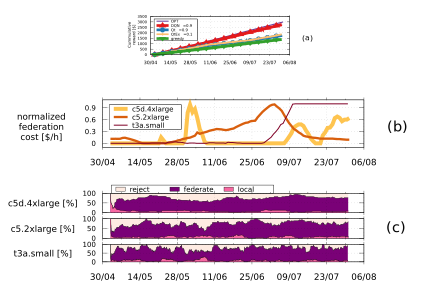
\includegraphics[width=\textwidth]{img/cdfs-all-decisions_edited_dqn-zoom-usage.pdf}}%
        \only<5>{\includegraphics[width=\textwidth]{img/cdfs-all-decisions_edited_dqn-zoom-usage-highlighter.pdf}}%
        \caption{Federation agents' performance.}
        \label{fig:cdf-dqn}
    \end{figure}
    \end{minipage}
\end{frame}





\begin{frame}
    \frametitle{\secname}
    \framesubtitle{\subsecname}

    \begin{figure}
        \centering
        \subfigure[Increasing local resources.]{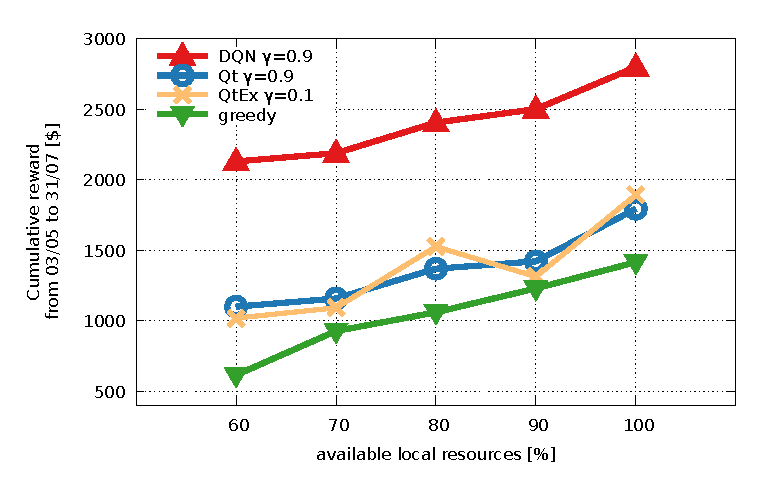
\includegraphics[width=.45\columnwidth]{img/shrink-local.eps}}\hspace{1em}
        \subfigure[Increasing resources in federation.]{\includegraphics[width=.45\columnwidth]{img/shrink-federated.eps}}
        \caption{Cumulative reward vs. available resources.}
    \end{figure}
\end{frame}








\subsection{Output}
\begin{frame}
    \frametitle{Outline}
    \tableofcontents[subsectionstyle=show/shaded/hide,sectionstyle=show/shaded]
\end{frame}

\begin{frame}
    \frametitle{\secname}
    \framesubtitle{\subsecname}
    Publications:
    \begin{itemize}
        \item \fullcite{multi-domain-msc}
        \item \fullcite{icc}
        \item \fullcite{dqn}
    \end{itemize}
\end{frame}




\begin{frame}
    \frametitle{\secname}
    \framesubtitle{\subsecname}
    Open-source:
    \begin{itemize}
        \item \textbf{DFS, BFS w/ cutoffs}: \url{https://github.com/MartinPJorge/placement/}
        \item \textbf{Q-table}: \url{https://github.com/MartinPJorge/5gt-federation/}
        \item \textbf{DQN \& environment}: \url{https://github.com/MartinPJorge/5gt-federation/tree/extensionICC/utils/aws/}
    \end{itemize}
\end{frame}







\section{NFV orchestration for 5G networks: OKpi}
\subsection{State of the art}
\begin{frame}
    \frametitle{Outline}
    \tableofcontents[subsectionstyle=show/shaded/hide,sectionstyle=show/shaded]
\end{frame}



\begin{frame}
    \frametitle{\secname}
    \framesubtitle{\subsecname}

    \begin{figure}
        \only<1>{\includegraphics[width=.6\textwidth]{img/fresco_var_thesis_scenario_base.pdf}}%
        \only<2>{\includegraphics[width=.6\textwidth]{img/fresco_var_thesis_scenario_cloud.pdf}}%
        \only<3>{\includegraphics[width=.6\textwidth]{img/fresco_var_thesis_scenario_edge.pdf}}%
        \only<4>{\includegraphics[width=.6\textwidth]{img/fresco_var_thesis_scenario_fog.pdf}}
        \caption{Virtual Network Function Embedding (VNE).}
    \end{figure}
\end{frame}






\begin{frame}
    \frametitle{\secname}
    \framesubtitle{\subsecname}

    Existing Virtual Network Embedding (VNE) solutions:
    \begin{itemize}
        \item latency-aware, bipartite graph \& Hungarian \cite{getting-the-most}
        \item maxZ: latency-aware, relaxed ILP~\cite{maxZ}
        \item z-TORCH: KPI monitoring, k-means VNF assign~\cite{z-TORCH}
        \item AIA: meet latency and throughput~\cite{adaptive-interference}
    \end{itemize}\pause
    \textbf{\color{red}OKpi} accounts for:
    \begin{itemize}
        \item latency constraints
        \item \textbf{\color{red}radio coverage}
        \item \textbf{\color{red}geographical availability}
        \item \textbf{\color{red}reliability}
    \end{itemize}
\end{frame}



\subsection{Thesis Contribution}
\begin{frame}
    \frametitle{Outline}
    \tableofcontents[subsectionstyle=show/shaded/hide,sectionstyle=show/shaded]
\end{frame}


\begin{frame}
    \frametitle{\secname}
    \framesubtitle{\subsecname}

    \begin{minipage}{0.37\textwidth}
        \textbf{Latency} constraint $D(s)$:
        \begin{equation}
            \only<1>{d_{\text{net}}(\psi) + d_{\text{proc}}(\psi) \le D(s)}
            \only<2>{\highlight{d_{\text{net}}(\psi)}{propagation delay} + d_{\text{proc}}(\psi) \le D(s)}
            \only<3>{d_{\text{net}}(\psi) + \highlight{d_{\text{proc}}(\psi)}{processing delay} \le D(s)}
            \label{eq:delay-constraint}
        \end{equation}
        \only<3>{$d_{\text{proc}}$: VNF as M/M/1-PS queue}
    \end{minipage}
    \begin{minipage}{0.6\textwidth}
        \begin{figure}
            \centering
            \only<1>{\includegraphics[width=.9\textwidth]{img/fresco_var_thesis_scenario_delay.pdf}}%
            \only<2>{\includegraphics[width=.9\textwidth]{img/fresco_var_thesis_scenario_propagation_delay.pdf}}%
            \only<3>{\includegraphics[width=.9\textwidth]{img/fresco_var_thesis_scenario_processing_delay.pdf}}%
            \caption{Service $s$ delay.}
        \end{figure}
    \end{minipage}
\end{frame}


\begin{frame}
    \frametitle{\secname}
    \framesubtitle{\subsecname}

    \begin{minipage}{0.5\textwidth}
        \textbf{Radio technology} $i$ constraint:
        \begin{equation}
            \rho(v , c)r_i (v) \le R_i (c)
            \label{eq:okpi-radio-constraint}
        \end{equation}
        \begin{itemize}
            \item $\rho(v,c)$: VNF $v$ is deployed in $c$ 
            \item $R_i (c)$: radio point of access c has radio technology $i$
            \item $r_i (v)$: VNF v needs radio technology $i$
        \end{itemize}
    \end{minipage}
    \begin{minipage}{0.45\textwidth}
        \begin{figure}
            \centering
            \includegraphics[width=.9\textwidth]{img/okpi-radio.pdf}
            \caption{Radio VNF.}
        \end{figure}
    \end{minipage}
\end{frame}





\begin{frame}
    \frametitle{\secname}
    \framesubtitle{\subsecname}

    \begin{minipage}{0.43\textwidth}
        \textbf{Geographical availability}:
        \begin{multline}
            \forall\psi = (\alpha, s), \exists c, v_1 , v_2:\\
            \tau_{\psi,c} (e, v_1 , v_2 ) > 0
            \label{eq:okpi-geo-constraint}
        \end{multline}
        \begin{itemize}
            \item location $\alpha$
            \item $\tau_{e,c} (e, v_1 , v_2 )$: flow $(\psi, v_1 , v_2 )$ traverses link $(\psi, c)$
        \end{itemize}
    \end{minipage}
    \begin{minipage}{0.55\textwidth}
        \begin{figure}
            \centering
            \includegraphics[width=.8\textwidth]{img/geographical.pdf}
            \caption{coverage of region $\alpha$.}
        \end{figure}
    \end{minipage}
\end{frame}





\begin{frame}
    \frametitle{\secname}
    \framesubtitle{\subsecname}

    \begin{minipage}{0.43\textwidth}
        Service \textbf{reliability} $H(s)$:
            \begin{multline}
                \only<1>{\prod_{\substack{ v_1,v_2\in\mathcal{V} \\ (i,j)\in w}}\eta(j,t)\eta(i,j,t)\geq H(s)}%
                \only<2>{\prod_{v_1,v_2\in\mathcal{V}}\sum_{w\in\mathcal{W}}\highlight{f(\psi,v_1,v_2,w)}{traffic fraction}\\\prod_{(i,j)\in w}\eta(j,t)\eta(i,j,t)\geq H(s)}
                \label{eq:okpi-reliab-constraint}
            \end{multline}
        \begin{itemize}
            \item $\eta(j,t)$: node reliability at $t$
            \item $\eta(i,j,t)$: node reliability at $t$
            \only<2>{\item $w$: traffic path}
        \end{itemize}
    \end{minipage}
    \hfill
    \begin{minipage}{0.50\textwidth}
        \begin{figure}
            \centering
            \only<1>{\includegraphics[width=.8\textwidth]{img/reliability-together.pdf}}%
            \only<2>{\includegraphics[width=.8\textwidth]{img/reliability-fraction.pdf}}%
            %\only<2>{\includegraphics[width=.8\textwidth]{img/reliability.pdf}}%
            \caption{
                \only<1>{Traffic path.}%
                \only<2>{Fractioned traffic path.}
            }
        \end{figure}
    \end{minipage}
\end{frame}






\begin{frame}
    \frametitle{\secname}
    \framesubtitle{\subsecname}

    Formulate an optimization problem:
    \begin{align}
        \label{eq:obj}
        \min &
        \only<1>{\sum_c\sum_{v} \left [ c_c(v)+\sum_{e}\sum_{\kappa}c_c(\kappa)a_c(\psi,v,\kappa) \right ]  +\sum_{(i,j)} \sum_{e} \sum_{v_1,v_2}c_{i,j}\tau_{i,j}(\psi,v_1,v_2)}%
        \only<2>{\sum_c\sum_{v} \Bigg[  \highlight{c_c(v)}{VNF cost}   +\sum_{e}\sum_{\kappa}c_c(\kappa)a_c(\psi,v,\kappa) \Bigg]  +\sum_{(i,j)} \sum_{e} \sum_{v_1,v_2}c_{i,j}\tau_{i,j}(\psi,v_1,v_2)}%
        \only<3>{\sum_c\sum_{v} \Bigg[  c_c(v)   +\sum_{e}\sum_{\kappa} \highlight{c_c(\kappa)a_c(\psi,v,\kappa)}{assigned resource $\kappa$ cost} \Bigg]  +\sum_{(i,j)} \sum_{e} \sum_{v_1,v_2}c_{i,j}\tau_{i,j}(\psi,v_1,v_2)}%
        \only<4>{\sum_c\sum_{v} \left [ c_c(v)+\sum_{e}\sum_{\kappa}c_c(\kappa)a_c(\psi,v,\kappa) \right ]  +\sum_{(i,j)} \sum_{e} \sum_{v_1,v_2}\highlight{c_{i,j}\tau_{i,j}(\psi,v_1,v_2)}{traffic steering cost}} %
        \only<5>{\sum_c\sum_{v} \left [ c_c(v)+\sum_{e}\sum_{\kappa}c_c(\kappa)a_c(\psi,v,\kappa) \right ]  +\sum_{(i,j)} \sum_{e} \sum_{v_1,v_2}c_{i,j}\tau_{i,j}(\psi,v_1,v_2)} \\
        s.t. & \eqref{eq:delay-constraint}-\eqref{eq:okpi-reliab-constraint}
    \end{align}
    \only<5>{NP-hard: bin-packing problem equivalence.}
\end{frame}





\begin{frame}
    \frametitle{\secname}
    \framesubtitle{\subsecname}

    The \textbf{OKpi} (all KPI) solution:
    \begin{itemize}
        \item infrastructure as a graph
        \item edges with:
            \begin{itemize}
                \item delay
                \item reliability
            \end{itemize}
    \end{itemize}
    \vfill\pause
    Solve in two steps:
    \begin{enumerate}
        \item Create a decision graph 
        \item Create an expanded graph
    \end{enumerate}
\end{frame}


\begin{frame}
    \frametitle{\secname}
    \framesubtitle{\subsecname}



    \begin{minipage}{.39\textwidth}
        \textbf{Decision graph} $\tilde{G}=(\tilde{N}, \tilde{E})$.\vspace{1em}
        
        \onslide<2->{Nodes $\tilde{N}=\{\tilde{n}_1, \tilde{n}_2, \ldots\}$:
            \begin{itemize}
                \item $|\mathcal{V}|-1$ replicas
            \end{itemize}
        }
        \vspace{1em}
        \onslide<3->{Edges $\tilde{E}=\{ (\tilde{n}_1,\tilde{n}_2),\ldots \}$:
            \begin{itemize}
                \item two weights:
                    \begin{equation}
                        \only<3>{\left( \frac{\tilde{D}_{\tilde{n}_1,\tilde{n}_2}}{D(s)}, \frac{\log \tilde{\eta}_{\tilde{n}_1,\tilde{n}_2}}{\log H(s)} \right)}%
                        \only<4>{\Bigg( \highlight{ \frac{\tilde{D}_{\tilde{n}_1,\tilde{n}_2}}{D(s)} }{delay fraction}, \frac{\log \tilde{\eta}_{\tilde{n}_1,\tilde{n}_2}}{\log H(s)} \Bigg)}%
                        \only<5>{\Bigg( \frac{\tilde{D}_{\tilde{n}_1,\tilde{n}_2}}{D(s)}, \highlight{ \frac{\log \tilde{\eta}_{\tilde{n}_1,\tilde{n}_2}}{\log H(s)} }{reliability fraction} \Bigg)}%
                        \onslide<6->{\left( \frac{\tilde{D}_{\tilde{n}_1,\tilde{n}_2}}{D(s)}, \frac{\log \tilde{\eta}_{\tilde{n}_1,\tilde{n}_2}}{\log H(s)} \right)}%
                    \end{equation}%
                \vspace{-1em}
                \onslide<6->{\item create links $(\tilde{n}_1,\tilde{n}_2)$}
            \end{itemize}
        }
    \end{minipage}
    \begin{minipage}{.6\textwidth}
        \begin{figure}
            \only<1>{\includegraphics[width=.8\textwidth]{img/decision-graph.pdf}}%
            \only<2>{\includegraphics[width=.8\textwidth]{img/decision-graph-replicas.pdf}}%
            \only<3>{\includegraphics[width=.8\textwidth]{img/decision-graph-replicas.pdf}}%
            \only<4>{\includegraphics[width=.8\textwidth]{img/decision-graph-replicas.pdf}}%
            \only<5>{\includegraphics[width=.8\textwidth]{img/decision-graph-replicas.pdf}}%
            % \only<6>{\includegraphics[width=.8\textwidth]{img/decision-graph-edges.pdf}}%
            \only<6>{\includegraphics[width=.8\textwidth]{img/decision-graph-edges-inter.pdf}}%
            \caption{OKpi decision graph.}
        \end{figure}
    \end{minipage}

\end{frame}






\begin{frame}
    \frametitle{\secname}
    \framesubtitle{\subsecname}

    \begin{minipage}{.39\textwidth}
        \textbf{Expanded graph}:

        \begin{enumerate}
            \item add superscripts $\tilde{n}^{d,r}$
                \begin{itemize}
                    \item $d$: delay to reach it
                    \item $r$: reliab. to reach it
                \end{itemize}
            \onslide<2->{\item add $(\gamma+1)^2$ replicas}
            \onslide<3->{\item connect $\tilde{n_1}^{d_1,r_2}$ with $\tilde{n_2}^{d_2,r_2}$}
                \onslide<4->{
                    \begin{itemize}
                        \item link $(\tilde{n}_1,\tilde{n}_2)\in\tilde{E}$
                        \item $d_1+\gamma\cdot d(\tilde{n}_1,\tilde{n}_2)\le d_2$
                        \item $r_1+\gamma\cdot r(\tilde{n}_1,\tilde{n}_2)\le r_2$
                    \end{itemize}
                }
            \onslide<5->{\item one hop per VNF}
        \end{enumerate}
    \end{minipage}
    \begin{minipage}{.6\textwidth}
        \begin{figure}
            \only<1>{\includegraphics[width=.8\textwidth]{img/expanded-one-node.pdf}}%
            \only<2>{\includegraphics[width=.8\textwidth]{img/expanded-one-node-replicas.pdf}}%
            \only<3>{\includegraphics[width=.8\textwidth]{img/expanded-all-connections.pdf}}%
            \only<4>{\includegraphics[width=.8\textwidth]{img/expanded-feasible-connections.pdf}}%
            \only<5>{\includegraphics[width=.8\textwidth]{img/expanded-solution-1.pdf}}%
            \only<6>{\includegraphics[width=.8\textwidth]{img/expanded-solution-2.pdf}}%
            \caption{OKpi expanded graph $\gamma=3$.}
        \end{figure}
    \end{minipage}
\end{frame}







\begin{frame}
    \frametitle{\secname}
    \framesubtitle{\subsecname}
    Simulations using realistic ITU+3GPP 5G scenarios~\cite{modelling-bs}:
    \begin{figure}[ht]
        \subfigure[]{ \includegraphics[height=.4\textheight]{img/robot-sfc}}\hspace{3em}
        \subfigure[]{ \includegraphics[height=.4\textheight]{img/increase-granularity}}
        \caption{(a) master-slave robotic VS illustration, and (b) optimality comparison of the VNFs' deployment costs using OKpi with $\gamma=3,10$.}
        \label{fig:fig}
    \end{figure}
\end{frame}


\begin{frame}
    \frametitle{\secname}
    \framesubtitle{\subsecname}

    Simulations using realistic ITU+3GPP 5G scenarios~\cite{modelling-bs}:
    \begin{figure}[ht]
        \subfigure[]{ \includegraphics[width=.35\textwidth]{img/delay-increase.png}}\hspace{2em}
        \subfigure[]{ \includegraphics[width=.35\textwidth]{img/traffic-increase.png}}
        \caption{(a) end-to-end delay, and (b) traffic impact on deployment cost of master-slave robotic VS.}
        \label{fig:increase-results}
    \end{figure}
\end{frame}











\subsection{Output}
\begin{frame}
    \frametitle{Outline}
    \tableofcontents[subsectionstyle=show/shaded/hide,sectionstyle=show/shaded]
\end{frame}


\begin{frame}
    \frametitle{\secname}
    \framesubtitle{\subsecname}
    Publications:
    \begin{itemize}
        \item \fullcite{okpi}
        \item \fullcite{okpi-ton}
        \item \fullcite{tmc}
    \end{itemize}
\end{frame}


\begin{frame}
    \frametitle{\secname}
    \framesubtitle{\subsecname}
    Open-source:
    \begin{itemize}
        \item \textbf{AMPLPY}: \url{https://github.com/ampl/amplpy/}
        \item \textbf{networkx}: \url{https://github.com/networkx/networkx/}
        \item \textbf{OKpi}: \url{https://github.com/MartinPJorge/placement/}
        \item \textbf{FMC}: \url{https://github.com/MartinPJorge/placement/}
    \end{itemize}
\end{frame}







\section{Scaling of V2N services: a study case}
\subsection{State of the art}
\begin{frame}
    \frametitle{Outline}
    \tableofcontents[subsectionstyle=show/shaded/hide,sectionstyle=show/shaded]
\end{frame}



\begin{frame}
    \frametitle{\secname}
    \framesubtitle{\subsecname}

    \begin{figure}
        \only<1>{\includegraphics[width=\textwidth]{img/v2n-scaling.pdf}}%
        \only<2>{\includegraphics[width=\textwidth]{img/v2n-scaling-2.pdf}}
        \caption{V2N service scaling.}
    \end{figure}

\end{frame}




\begin{frame}
    \frametitle{\secname}
    \framesubtitle{\subsecname}

    V2N scaling solutions:
    \begin{itemize}
        \item asign radio resource blocks~\cite{pi-road}
        \item computing resources scaling:
            \begin{itemize}
                \item threshold-based~\cite{5gt-v2x,luis-v2x}
                \item LSTM-based~\cite{automec}
                \pause
                {\color{red}\item  \textbf{compare}:
                    \begin{itemize}
                        \item \color{red} DES, TES
                        \item \color{red} HTM
                        \item \color{red} GRU
                        \item \color{red} LSTM
                        \item \color{red} TCN
                        \item \color{red} TCNLSTM
                    \end{itemize}
                }
            \end{itemize}
    \end{itemize}
\end{frame}





\subsection{Thesis contribution}
\begin{frame}
    \frametitle{Outline}
    \tableofcontents[subsectionstyle=show/shaded/hide,sectionstyle=show/shaded]
\end{frame}


\begin{frame}
    \frametitle{\secname}
    \framesubtitle{\subsecname}

    \begin{figure}
        \includegraphics[width=\textwidth]{img/v2n-scaling-scenario.pdf}
        \caption{V2N service vertical scaling.}
    \end{figure}
\end{frame}





\begin{frame}
    \frametitle{\secname}
    \framesubtitle{\subsecname}

    \begin{minipage}{0.37\textwidth}
        Edge server -- $M/M/c$ queue:
        \begin{itemize}
            \item $\lambda(t)$: cars' arrival rate
            \item $\mu$: CPU service rate
            \item $c(t)$: number of CPUs
        \end{itemize}
        \only<2>{Scale to meet avg. latency:
            \begin{equation}
                \frac{1}{\mu} + \frac{P_Q}{c(t)\mu - \lambda(t)}
            \end{equation}
            with $P_Q$ the prob. of all servers bussy (Earlang C).
        }
    \end{minipage}
    \hfill
    \begin{minipage}{0.6\textwidth}
        \begin{figure}
            \centering
            \includegraphics[width=.8\textwidth]{img/MMc.pdf}
            \caption{Server as $M/M/c$ queue.}
        \end{figure}
    \end{minipage}
\end{frame}




\begin{frame}
    \frametitle{\secname}
    \framesubtitle{\subsecname}

    \begin{minipage}{0.37\textwidth}
        \textbf{Dataset} to derive $\lambda(t)$:
        \begin{itemize}
            \item 116 roads in Torino
            \item (lat,lng) of roads
            \item traffic [vehicles/hour] each 5 min.
            \item avg. speed [vehicles/hour] each 5 min.
            \item from 28/01/2020 -- now
        \end{itemize}
    \end{minipage}
    \hfill
    \begin{minipage}{0.6\textwidth}
        \begin{figure}
            \centering
            \includegraphics[width=.9\textwidth]{img/traffic-drop.pdf}
            \caption{Traffic after COVID-19 lockdowns -- 8~March.}
        \end{figure}
    \end{minipage}
\end{frame}





\begin{frame}
    \frametitle{\secname}
    \framesubtitle{\subsecname}

    \begin{figure}
        \animategraphics[autoplay,loop,trim = 0 100px 0 100px, width=.6\textwidth]{10}{img/torino-traffic-}{0}{27}
        \caption{Vehicular traffic -- wee hours @Torino.}
    \end{figure}
\end{frame}





\begin{frame}
    \frametitle{\secname}
    \framesubtitle{\subsecname}

    \begin{minipage}{0.37\textwidth}
        Predict future traffic $\lambda(t+n)$
        \begin{itemize}
            \item \textbf{time-series techniques}: DES, TES
            \item \textbf{proprietary}: HTM
            \item \textbf{neural networks}: GRU, LSTM, TCN, TCNLSTM
        \end{itemize}
        
        Patterns:
        \begin{itemize}
            \item strong \textbf{seasonality}.
            \onslide<2->{\item week \& weekend flows}
            \item \onslide<3->{night hours,} \onslide<4->{rush hours,} \onslide<5->{schools' out}
        \end{itemize}
    \end{minipage}
    \hfill
    \begin{minipage}{0.6\textwidth}
        \begin{figure}
            \centering
            \only<1>{\includegraphics[width=.9\textwidth]{img/orbassano-flow.pdf}}%
            \only<2>{\includegraphics[width=.9\textwidth]{img/orbassano-flow-annotate-weekend.pdf}}%
            \only<3>{\includegraphics[width=.9\textwidth]{img/orbassano-flow-annotate-night.pdf}}%
            \only<4>{\includegraphics[width=.9\textwidth]{img/orbassano-flow-annotate-rush.pdf}}%
            \only<5>{\includegraphics[width=.9\textwidth]{img/orbassano-flow-annotate-shools-out.pdf}}%
            \caption{Weekly traffic at Corso Orbassano road.}
        \end{figure}
    \end{minipage}
\end{frame}





\begin{frame}
    \frametitle{\secname}
    \framesubtitle{\subsecname}

    \begin{minipage}{0.37\textwidth}
            \textbf{non-COVID-19} (2020)
                \begin{itemize}
                    \item training: 28\textsuperscript{th}Feb - 28\textsuperscript{th}Mar
                    \item testing: 29\textsuperscript{th}Feb - 07\textsuperscript{th}Mar
                \end{itemize}
            \textbf{COVID-19} (2020)
                \begin{itemize}
                    \item training: 06\textsuperscript{th}Feb - 07\textsuperscript{th}Mar
                    \item testing: 08\textsuperscript{th}Mar - 15\textsuperscript{th}Mar
                \end{itemize}
        \vspace{1.5em}
        \onslide<2->{\textbf{Train}:
            \begin{itemize}
                \item offline training
                \item online training
            \end{itemize}
        }
    \end{minipage}
    \hfill
    \begin{minipage}{0.6\textwidth}
        \only<2->{\begin{figure}
                \centering
                \includegraphics[width=.9\textwidth]{img/online-training-high-res.pdf}%
                \caption{Online training.}
            \end{figure}
        }
    \end{minipage}

\end{frame}




\begin{frame}
    \frametitle{\secname}
    \framesubtitle{\subsecname}

    \begin{minipage}{0.37\textwidth}
        \textbf{Vertical scaling}:
        \begin{enumerate}
            \item $\lambda(t+n)$: traffic prediction
            \only<2>{\item derive $c(t+n)$ s.t.:
                \begin{equation}
                    \frac{1}{\mu} + \frac{P_Q}{c(t+n)\mu-\lambda(t+n)}\le D(s)
                \end{equation}
                with $D(s)$ the target delay
            }
        \end{enumerate}
    \end{minipage}
    \hfill
    \begin{minipage}{0.6\textwidth}
        \begin{figure}
            \centering
            \only<1>{\includegraphics[width=.9\textwidth]{img/MMc-scaling-1.pdf}}%
            \only<2>{\includegraphics[width=.9\textwidth]{img/MMc-scaling.pdf}}
            \caption{$M/M/c$-based scaling.}
        \end{figure}
    \end{minipage}
\end{frame}






\begin{frame}
    \frametitle{\secname}
    \framesubtitle{\subsecname}

    \center{{\color{white}\_}\only<2>{Most accurate: \color{red}\textbf{Neural Networks}}}

    \begin{figure}
        \centering
        \subfigure[][non-COVID-19]{%
            \only<1>{\includegraphics[width=.49\textwidth]{img/draft-non-covid-offline-steps.pdf}}%
            \only<2>{\includegraphics[width=.49\textwidth]{img/draft-non-covid-offline-steps-winner.pdf}}%
            \label{fig:offline-non-covid-steps}%
        }%
        %\hspace{8pt}
        \subfigure[][COVID-19]{%
            \only<1>{\includegraphics[width=.49\textwidth]{img/draft-covid-offline-steps.pdf}}%
            \only<2>{\includegraphics[width=.49\textwidth]{img/draft-covid-offline-steps-winner.pdf}}%
            \label{fig:offline-covid-steps}%
        }
        \centering
        \caption[]{
            Prediction accuracy (offline training).
        }%
    \end{figure}
\end{frame}







\begin{frame}
    \frametitle{\secname}
    \framesubtitle{\subsecname}

    \center{{\color{white}\_}\only<2>{Most accurate: \color{red}\textbf{TES}}}

    \begin{figure}
        \centering
        \subfigure[][non-COVID-19]{%
            \only<1>{\includegraphics[width=.49\textwidth]{img/draft-non-covid-online-steps.pdf}}%
            \only<2>{\includegraphics[width=.49\textwidth]{img/draft-non-covid-online-steps-winner.pdf}}%
            \label{fig:online-non-covid-steps}%
        }%
        %\hspace{8pt}%
        \subfigure[][COVID-19]{%
            \only<1>{\includegraphics[width=.49\textwidth]{img/draft-covid-online-steps.pdf}}%
            \only<2>{\includegraphics[width=.49\textwidth]{img/draft-covid-online-steps-winner.pdf}}%
            \label{fig:online-covid-steps}%
        }%
        \centering
        \caption[]{
            Prediction accuracy (online training).
        }%
    \end{figure}
\end{frame}





%%%%%    \begin{frame}
%%%%%        \frametitle{\secname}
%%%%%        \framesubtitle{\subsecname}
%%%%%    
%%%%%        \begin{figure}
%%%%%            \centering
%%%%%            \only<1>{
%%%%%                \subfigure[][Remote driving savings]{%
%%%%%                    \includegraphics[width=.3\textwidth]{img/draft-remote-driving-cost.pdf}%
%%%%%                    \label{fig:cost-remote}%
%%%%%                }%
%%%%%                \subfigure[][Coop. aware. savings]{%
%%%%%                    \includegraphics[width=.3\textwidth]{img/draft-cooperative-awareness-cost.pdf}%
%%%%%                    \label{fig:cost-cooperative}%
%%%%%                }%
%%%%%                \subfigure[][Hazard warn. savings]{%
%%%%%                    \includegraphics[width=.3\textwidth]{img/draft-hazard-warning-cost.pdf}%
%%%%%                    \label{fig:cost-hazard}%
%%%%%                }\\%
%%%%%                \subfigure[][Remote driving delay violate]{%
%%%%%                    \includegraphics[width=.3\textwidth]{img/draft-remote-driving-delay-violations.pdf}%
%%%%%                    \label{fig:delay-remote}%
%%%%%                }%
%%%%%                \subfigure[][Coop. aware. delay violate]{%
%%%%%                    \includegraphics[width=.3\textwidth]{img/draft-cooperative-awareness-delay-violations.pdf}%
%%%%%                    \label{fig:delay-cooperative}%
%%%%%                }%
%%%%%                \subfigure[][Hazard warn. violate]{%
%%%%%                    \includegraphics[width=.3\textwidth]{img/draft-hazard-warning-delay-violations.pdf}%
%%%%%                    \label{fig:delay-hazard}%
%%%%%                }%
%%%%%            }%
%%%%%            \only<2>{
%%%%%                \subfigure[][Remote driving savings]{%
%%%%%                    \includegraphics[width=.3\textwidth]{img/draft-remote-driving-cost-highlight.pdf}%
%%%%%                    \label{fig:cost-remote}%
%%%%%                }%
%%%%%                \subfigure[][Coop. aware. savings]{%
%%%%%                    \includegraphics[width=.3\textwidth]{img/draft-cooperative-awareness-cost.pdf}%
%%%%%                    \label{fig:cost-cooperative}%
%%%%%                }%
%%%%%                \subfigure[][Hazard warn. savings]{%
%%%%%                    \includegraphics[width=.3\textwidth]{img/draft-hazard-warning-cost.pdf}%
%%%%%                    \label{fig:cost-hazard}%
%%%%%                }\\
%%%%%                \subfigure[][Remote driving delay violate]{%
%%%%%                    \includegraphics[width=.3\textwidth]{img/draft-remote-driving-delay-violations-highlight.pdf}%
%%%%%                    \label{fig:delay-remote}%
%%%%%                }%
%%%%%                \subfigure[][Coop. aware. delay violate]{%
%%%%%                    \includegraphics[width=.3\textwidth]{img/draft-cooperative-awareness-delay-violations.pdf}%
%%%%%                    \label{fig:delay-cooperative}%
%%%%%                }%
%%%%%                \subfigure[][Hazard warn. violate]{%
%%%%%                    \includegraphics[width=.3\textwidth]{img/draft-hazard-warning-delay-violations.pdf}%
%%%%%                    \label{fig:delay-hazard}%
%%%%%                }%
%%%%%            }%
%%%%%            \only<3>{
%%%%%                \subfigure[][Remote driving savings]{%
%%%%%                    \includegraphics[width=.3\textwidth]{img/draft-remote-driving-cost.pdf}%
%%%%%                    \label{fig:cost-remote}%
%%%%%                }%
%%%%%                \subfigure[][Coop. aware. savings]{%
%%%%%                    \includegraphics[width=.3\textwidth]{img/draft-cooperative-awareness-cost-highlight.pdf}%
%%%%%                    \label{fig:cost-cooperative}%
%%%%%                }%
%%%%%                \subfigure[][Hazard warn. savings]{%
%%%%%                    \includegraphics[width=.3\textwidth]{img/draft-hazard-warning-cost.pdf}%
%%%%%                    \label{fig:cost-hazard}%
%%%%%                }\\%
%%%%%                \subfigure[][Remote driving delay violate]{%
%%%%%                    \includegraphics[width=.3\textwidth]{img/draft-remote-driving-delay-violations.pdf}%
%%%%%                    \label{fig:delay-remote}%
%%%%%                }%
%%%%%                \subfigure[][Coop. aware. delay violate]{%
%%%%%                    \includegraphics[width=.3\textwidth]{img/draft-cooperative-awareness-delay-violations-highlight.pdf}%
%%%%%                    \label{fig:delay-cooperative}%
%%%%%                }%
%%%%%                \subfigure[][Hazard warn. violate]{%
%%%%%                    \includegraphics[width=.3\textwidth]{img/draft-hazard-warning-delay-violations.pdf}%
%%%%%                    \label{fig:delay-hazard}%
%%%%%                }%
%%%%%            }%
%%%%%            \only<4>{
%%%%%                \subfigure[][Remote driving savings]{%
%%%%%                    \includegraphics[width=.3\textwidth]{img/draft-remote-driving-cost.pdf}%
%%%%%                    \label{fig:cost-remote}%
%%%%%                }%
%%%%%                \subfigure[][Coop. aware. savings]{%
%%%%%                    \includegraphics[width=.3\textwidth]{img/draft-cooperative-awareness-cost.pdf}%
%%%%%                    \label{fig:cost-cooperative}%
%%%%%                }%
%%%%%                \subfigure[][Hazard warn. savings]{%
%%%%%                    \includegraphics[width=.3\textwidth]{img/draft-hazard-warning-cost-highlight.pdf}%
%%%%%                    \label{fig:cost-hazard}%
%%%%%                }\\%
%%%%%                \subfigure[][Remote driving delay violate]{%
%%%%%                    \includegraphics[width=.3\textwidth]{img/draft-remote-driving-delay-violations.pdf}%
%%%%%                    \label{fig:delay-remote}%
%%%%%                }%
%%%%%                \subfigure[][Coop. aware. delay violate]{%
%%%%%                    \includegraphics[width=.3\textwidth]{img/draft-cooperative-awareness-delay-violations.pdf}%
%%%%%                    \label{fig:delay-cooperative}%
%%%%%                }%
%%%%%                \subfigure[][Hazard warn. violate]{%
%%%%%                    \includegraphics[width=.3\textwidth]{img/draft-hazard-warning-delay-violations-highlight.pdf}%
%%%%%                    \label{fig:delay-hazard}%
%%%%%                }%
%%%%%            }%
%%%%%            \caption[]{
%%%%%                Cost savings and delay violations due to scaling --
%%%%%                TES with online training was used.
%%%%%            }%
%%%%%        \end{figure}
%%%%%    \end{frame}







\begin{frame}
    \frametitle{\secname}
    \framesubtitle{\subsecname}

    \begin{figure}
        \centering
            \subfigure[][Remote driving savings]{%
                \includegraphics<1>[width=.3\textwidth]{img/draft-remote-driving-cost.pdf}%
                \includegraphics<2>[width=.3\textwidth]{img/draft-remote-driving-cost-highlight.pdf}%
                \includegraphics<3->[width=.3\textwidth]{img/draft-remote-driving-cost.pdf}%
                \label{fig:cost-remote}%
            }%
            \subfigure[][Coop. aware. savings]{%
                \includegraphics<1>[width=.3\textwidth]{img/draft-cooperative-awareness-cost.pdf}%
                \includegraphics<2>[width=.3\textwidth]{img/draft-cooperative-awareness-cost.pdf}%
                \includegraphics<3>[width=.3\textwidth]{img/draft-cooperative-awareness-cost-highlight.pdf}%
                \includegraphics<4>[width=.3\textwidth]{img/draft-cooperative-awareness-cost.pdf}%
                \label{fig:cost-cooperative}%
            }%
            \subfigure[][Hazard warn. savings]{%
                \includegraphics<1>[width=.3\textwidth]{img/draft-hazard-warning-cost.pdf}%
                \includegraphics<2>[width=.3\textwidth]{img/draft-hazard-warning-cost.pdf}%
                \includegraphics<3>[width=.3\textwidth]{img/draft-hazard-warning-cost.pdf}%
                \includegraphics<4>[width=.3\textwidth]{img/draft-hazard-warning-cost-highlight.pdf}%
                \label{fig:cost-hazard}%
            }\\%
            \subfigure[][Remote driving delay violate]{%
                \includegraphics<1>[width=.3\textwidth]{img/draft-remote-driving-delay-violations.pdf}%
                \includegraphics<2>[width=.3\textwidth]{img/draft-remote-driving-delay-violations-highlight.pdf}%
                \includegraphics<3->[width=.3\textwidth]{img/draft-remote-driving-delay-violations.pdf}%
                \label{fig:delay-remote}%
            }%
            \subfigure[][Coop. aware. delay violate]{%
                \includegraphics<1>[width=.3\textwidth]{img/draft-cooperative-awareness-delay-violations.pdf}%
                \includegraphics<2>[width=.3\textwidth]{img/draft-cooperative-awareness-delay-violations.pdf}%
                \includegraphics<3>[width=.3\textwidth]{img/draft-cooperative-awareness-delay-violations-highlight.pdf}%
                \includegraphics<4>[width=.3\textwidth]{img/draft-cooperative-awareness-delay-violations.pdf}%
                \label{fig:delay-cooperative}%
            }%
            \subfigure[][Hazard warn. violate]{%
                \includegraphics<1>[width=.3\textwidth]{img/draft-hazard-warning-delay-violations.pdf}%
                \includegraphics<2>[width=.3\textwidth]{img/draft-hazard-warning-delay-violations.pdf}%
                \includegraphics<3>[width=.3\textwidth]{img/draft-hazard-warning-delay-violations.pdf}%
                \includegraphics<4>[width=.3\textwidth]{img/draft-hazard-warning-delay-violations-highlight.pdf}%
                \label{fig:delay-hazard}%
            }%
        \caption[]{
            Cost savings and delay violations due to scaling --
            TES with online training was used.
        }%
    \end{figure}
\end{frame}







%%%%%    %% COUNTER FOR CURRENT FRAME & FIGURE
%%%%%    \newcounter{currframe}
%%%%%    \setcounter{currframe}{\value{framenumber}}
%%%%%    \newcounter{currfig}
%%%%%    \setcounter{currfig}{\value{figure}}
%%%%%    
%%%%%    
%%%%%    \begin{frame}
%%%%%        \frametitle{\secname}
%%%%%        \framesubtitle{\subsecname}
%%%%%    
%%%%%    
%%%%%        \begin{figure}
%%%%%            \subfigure[][Remote driving savings]{%
%%%%%                \includegraphics[width=.3\textwidth]{img/draft-remote-driving-cost.pdf}%
%%%%%                \label{fig:cost-remote}%
%%%%%            }%
%%%%%            \subfigure[][Coop. aware. savings]{%
%%%%%                \includegraphics[width=.3\textwidth]{img/draft-cooperative-awareness-cost.pdf}%
%%%%%                \label{fig:cost-cooperative}%
%%%%%            }%
%%%%%            \subfigure[][Hazard warn. savings]{%
%%%%%                \includegraphics[width=.3\textwidth]{img/draft-hazard-warning-cost.pdf}%
%%%%%                \label{fig:cost-hazard}%
%%%%%            }\\%
%%%%%            \subfigure[][Remote driving delay violate]{%
%%%%%                \includegraphics[width=.3\textwidth]{img/draft-remote-driving-delay-violations.pdf}%
%%%%%                \label{fig:delay-remote}%
%%%%%            }%
%%%%%            \subfigure[][Coop. aware. delay violate]{%
%%%%%                \includegraphics[width=.3\textwidth]{img/draft-cooperative-awareness-delay-violations.pdf}%
%%%%%                \label{fig:delay-cooperative}%
%%%%%            }%
%%%%%            \subfigure[][Hazard warn. violate]{%
%%%%%                \includegraphics[width=.3\textwidth]{img/draft-hazard-warning-delay-violations.pdf}%
%%%%%                \label{fig:delay-hazard}%
%%%%%            }%
%%%%%    
%%%%%            \caption[]{
%%%%%                Cost savings and delay violations due to scaling --
%%%%%                TES with online training was used.
%%%%%            }%
%%%%%        \end{figure}
%%%%%    \end{frame}
%%%%%    \setcounter{framenumber}{\value{currframe}}
%%%%%    \setcounter{figure}{\value{currfig}}
%%%%%    
%%%%%    
%%%%%    %% 2
%%%%%    \begin{frame}
%%%%%        \frametitle{\secname}
%%%%%        \framesubtitle{\subsecname}
%%%%%    
%%%%%    
%%%%%        \begin{figure}
%%%%%            \subfigure[][Remote driving savings]{%
%%%%%                \includegraphics[width=.3\textwidth]{img/draft-remote-driving-cost-highlight.pdf}%
%%%%%                \label{fig:cost-remote}%
%%%%%            }%
%%%%%            \subfigure[][Coop. aware. savings]{%
%%%%%                \includegraphics[width=.3\textwidth]{img/draft-cooperative-awareness-cost.pdf}%
%%%%%                \label{fig:cost-cooperative}%
%%%%%            }%
%%%%%            \subfigure[][Hazard warn. savings]{%
%%%%%                \includegraphics[width=.3\textwidth]{img/draft-hazard-warning-cost.pdf}%
%%%%%                \label{fig:cost-hazard}%
%%%%%            }\\
%%%%%            \subfigure[][Remote driving delay violate]{%
%%%%%                \includegraphics[width=.3\textwidth]{img/draft-remote-driving-delay-violations-highlight.pdf}%
%%%%%                \label{fig:delay-remote}%
%%%%%            }%
%%%%%            \subfigure[][Coop. aware. delay violate]{%
%%%%%                \includegraphics[width=.3\textwidth]{img/draft-cooperative-awareness-delay-violations.pdf}%
%%%%%                \label{fig:delay-cooperative}%
%%%%%            }%
%%%%%            \subfigure[][Hazard warn. violate]{%
%%%%%                \includegraphics[width=.3\textwidth]{img/draft-hazard-warning-delay-violations.pdf}%
%%%%%                \label{fig:delay-hazard}%
%%%%%            }%
%%%%%    
%%%%%            \caption[]{
%%%%%                Cost savings and delay violations due to scaling --
%%%%%                TES with online training was used.
%%%%%            }%
%%%%%        \end{figure}
%%%%%    \end{frame}
%%%%%    \setcounter{framenumber}{\value{currframe}}
%%%%%    \setcounter{figure}{\value{currfig}}
%%%%%    
%%%%%    
%%%%%    %% 3
%%%%%    \begin{frame}
%%%%%        \frametitle{\secname}
%%%%%        \framesubtitle{\subsecname}
%%%%%    
%%%%%    
%%%%%        \begin{figure}
%%%%%            \subfigure[][Remote driving savings]{%
%%%%%                \includegraphics[width=.3\textwidth]{img/draft-remote-driving-cost.pdf}%
%%%%%                \label{fig:cost-remote}%
%%%%%            }%
%%%%%            \subfigure[][Coop. aware. savings]{%
%%%%%                \includegraphics[width=.3\textwidth]{img/draft-cooperative-awareness-cost-highlight.pdf}%
%%%%%                \label{fig:cost-cooperative}%
%%%%%            }%
%%%%%            \subfigure[][Hazard warn. savings]{%
%%%%%                \includegraphics[width=.3\textwidth]{img/draft-hazard-warning-cost.pdf}%
%%%%%                \label{fig:cost-hazard}%
%%%%%            }\\%
%%%%%            \subfigure[][Remote driving delay violate]{%
%%%%%                \includegraphics[width=.3\textwidth]{img/draft-remote-driving-delay-violations.pdf}%
%%%%%                \label{fig:delay-remote}%
%%%%%            }%
%%%%%            \subfigure[][Coop. aware. delay violate]{%
%%%%%                \includegraphics[width=.3\textwidth]{img/draft-cooperative-awareness-delay-violations-highlight.pdf}%
%%%%%                \label{fig:delay-cooperative}%
%%%%%            }%
%%%%%            \subfigure[][Hazard warn. violate]{%
%%%%%                \includegraphics[width=.3\textwidth]{img/draft-hazard-warning-delay-violations.pdf}%
%%%%%                \label{fig:delay-hazard}%
%%%%%            }%
%%%%%    
%%%%%            \caption[]{
%%%%%                Cost savings and delay violations due to scaling --
%%%%%                TES with online training was used.
%%%%%            }%
%%%%%        \end{figure}
%%%%%    \end{frame}
%%%%%    \setcounter{framenumber}{\value{currframe}}
%%%%%    \setcounter{figure}{\value{currfig}}
%%%%%    
%%%%%    
%%%%%    %% 4
%%%%%    \begin{frame}
%%%%%        \frametitle{\secname}
%%%%%        \framesubtitle{\subsecname}
%%%%%    
%%%%%    
%%%%%        \begin{figure}
%%%%%            \subfigure[][Remote driving savings]{%
%%%%%                \includegraphics[width=.3\textwidth]{img/draft-remote-driving-cost.pdf}%
%%%%%                \label{fig:cost-remote}%
%%%%%            }%
%%%%%            \subfigure[][Coop. aware. savings]{%
%%%%%                \includegraphics[width=.3\textwidth]{img/draft-cooperative-awareness-cost.pdf}%
%%%%%                \label{fig:cost-cooperative}%
%%%%%            }%
%%%%%            \subfigure[][Hazard warn. savings]{%
%%%%%                \includegraphics[width=.3\textwidth]{img/draft-hazard-warning-cost-highlight.pdf}%
%%%%%                \label{fig:cost-hazard}%
%%%%%            }\\%
%%%%%            \subfigure[][Remote driving delay violate]{%
%%%%%                \includegraphics[width=.3\textwidth]{img/draft-remote-driving-delay-violations.pdf}%
%%%%%                \label{fig:delay-remote}%
%%%%%            }%
%%%%%            \subfigure[][Coop. aware. delay violate]{%
%%%%%                \includegraphics[width=.3\textwidth]{img/draft-cooperative-awareness-delay-violations.pdf}%
%%%%%                \label{fig:delay-cooperative}%
%%%%%            }%
%%%%%            \subfigure[][Hazard warn. violate]{%
%%%%%                \includegraphics[width=.3\textwidth]{img/draft-hazard-warning-delay-violations-highlight.pdf}%
%%%%%                \label{fig:delay-hazard}%
%%%%%            }%
%%%%%    
%%%%%            \caption[]{
%%%%%                Cost savings and delay violations due to scaling --
%%%%%                TES with online training was used.
%%%%%            }%
%%%%%        \end{figure}
%%%%%    \end{frame}








\subsection{Output}
\begin{frame}
    \frametitle{Outline}
    \tableofcontents[subsectionstyle=show/shaded/hide,sectionstyle=show/shaded]
\end{frame}

\begin{frame}
    \frametitle{\secname}
    \framesubtitle{\subsecname}
    Publications:
    \begin{itemize}
        \item \fullcite{eucnc-v2n}
        \item \fullcite{v2n-access}
    \end{itemize}

    Open-source (to be released):
    \begin{itemize}
        \item \url{https://github.com/MartinPJorge/5growth-scaling/}
        \item \url{https://github.com/MartinPJorge/5growth-forecasting/}
    \end{itemize}
\end{frame}



\section{Conclusions \& future work}
\begin{frame}
    \frametitle{Outline}
    \tableofcontents[subsectionstyle=show/shaded/hide,sectionstyle=show/shaded]
\end{frame}

%%% OLD CONCLUSIONS
%% \begin{frame}
%%     \frametitle{\secname}
%%     \framesubtitle{Conclusions}
%%     \begin{enumerate}
%%         \item methodology to \textbf{generate BS \& MEC PoP} locations\pause
%%         \item \textbf{DQN} agent to \textbf{federate} services under \textbf{dynamic prices}\pause
%%         \item \textbf{OKpi} solves VNE problem \& meets: delay, reliability, availability\pause
%%         \item \textbf{V2N scaling} w/ \textbf{TES} reduces delay violations using \textbf{online training}
%%     \end{enumerate}
%% \end{frame}




\begin{frame}
    \frametitle{\secname}
    \framesubtitle{Conclusions}
    In the \textbf{NFV orchestration} process, this thesis contributes to:\pause
    \begin{enumerate}
        \item generate \textbf{5G graphs} meeting standard requirements\pause
        \item maximize revenue under \textbf{federation} and dynamic pricing\pause
        \item minimize \textbf{VNE} cost meeting: latency, reliability, and availability constraints\pause
        \item reduce the E2E latency violations with the proposed \textbf{scaling}
    \end{enumerate}
\end{frame}






\begin{frame}
    \frametitle{\secname}
    \framesubtitle{Future work}
    \begin{enumerate}
        \item \textbf{generate federated} scenarios BSs, PoPs \& datacenters, all at once\pause
        \item \textbf{DQN} agent +\textbf{LSTM} layer to \textbf{predict}\pause
        \item \textbf{OKpi} study on $\gamma$/runtime/optimality \pause
        \item \textbf{V2N scaling} to meet \textbf{99.9999\%} latency quantile \& use \textbf{ST-GCN}
    \end{enumerate}
\end{frame}



\section*{Thesis publications}
\subsection*{Conferences}
\begin{frame}[allowframebreaks]
    \frametitle{\secname}
    \framesubtitle{\subsecname}

    \begin{itemize}
        \item \fullcite{multi-domain-msc}
        \item \fullcite{5gen}
        \item \fullcite{okpi}
        \item \fullcite{icc}
        \item \fullcite{eucnc-v2n}
    \end{itemize}
\end{frame}


\subsection*{Journals}
\begin{frame}[allowframebreaks]
    \frametitle{\secname}
    \framesubtitle{\subsecname}
    \begin{itemize}
        \item \fullcite{modelling-bs}
        \item \fullcite{tmc}
        \item \fullcite{dqn}
        \item \fullcite{okpi-ton}
    \end{itemize}
\end{frame}






\begin{frame}
    \frametitle{Thanks}

    \center{\huge
        Thanks for your attention!
    }
\end{frame}






\section*{References}
\begin{frame}[allowframebreaks]
        \frametitle{References}
        % \bibliographystyle{amsalpha}
        % \bibliography{bibliography.bib}
        \printbibliography[heading=none]
\end{frame}







\section*{Appendix}
\begin{frame}
    \frametitle{\secname}
    \framesubtitle{Inhomogeneous Mattérn~II process}
    \begin{lemma}
    Given an \emph{inhomogeneous} marked PPP $X$ with \emph{intensity function} $\lambda$, the \emph{thinning} function $I_2$, and marks $m \sim \frac{1}{\lambda(x)}$, the resulting thinned point process, called \emph{inhomogeneous Mat\'ern~II}~PP, has the following average \emph{number of points} at $C$:
        \begin{equation}
            \mathbb{E}\left[ N(C) \right] := \int_C e^{-\int_{B(x,r)} \mathds{1}\left(\lambda(u) > \lambda(x) \right) \lambda(u) du} \lambda(x)\ dx
            \label{eq:inh-matern2-avg}
        \end{equation}
        where $r$ is the \emph{thinning} radius of $I_2$.
        \label{prop:inh-matern2-avg}
    \end{lemma}



    \vfill
    with
    \begin{equation}
        I_2(x,m, X, M_X) := \begin{cases*}
            1 & if $m = \min_{m' \in M_X}\big\{ (x',m'): x'\in B(x,r) \big\}$\\
            0 & otherwise
        \end{cases*}
        \label{eq:matern2}
    \end{equation}

\end{frame}





\begin{frame}
    \frametitle{\secname}
    \framesubtitle{Maximum distance between PoP and BS}


    The RTT considered is computed as
    \begin{equation}
        RTT := 2 l\left(\lVert x - m \rVert_1 \right) + 2 p(M) + UL + DL
        \label{eq:rtt}
    \end{equation}


    We find $m_M$, the maximum distance from MEC PoP $m$ to the BS at position $x$, as:
    \begin{equation}
        \lVert x-m \rVert_1 \le l^{-1}\left( \frac{RTT - 2p(M) - t_r}{2} \right)  = m_M
        \label{eq:max-dis}
    \end{equation}
    with $\lVert \cdot \rVert_1$ denoting the Manhattan distance.
\end{frame}




\begin{frame}
    \frametitle{\secname}
    \framesubtitle{Pricing details}

    \textbf{User pays} $p^{(t)}$ for the service $\sigma$
    \begin{equation}
        \mbox{$p^{(t)}(\sigma)=(1+P)l^{(t)}(\sigma)$}
        \label{eq:service-fee}
    \end{equation}
    with $P$ the profit margin, and $l^{(t)}$ the local deployment cost (based on uncertain phenomena).\pause 

    \vfill

    Given the federation fee $f(\sigma)$ the \textbf{reward} is:
    \begin{equation}
        r^{(t)}(X_t) := \!\!\!\!\!\!\!\!\!\!\sum_{\substack{\sigma:~ x(\sigma)=0\\a(\sigma) \le t\le d(\sigma)}} \!\!\!\!\!\!\!\! p^{a(\sigma)}(\sigma) +\!\!\!\!\!\!\!\!\!\! \sum_{\substack{\sigma:~ x(\sigma)=1\\ a(\sigma) \le t\le d(\sigma)}} \!\!\!\!\!\!\!\!\left[ p^{a(\sigma)}(\sigma) - f^{(t)}(\sigma) \right]
        \label{eq:instant-reward}
    \end{equation}
    where $X_t:=\{ x(\sigma) \}_{\sigma: a(\sigma)\le t}$.

\end{frame}



















\begin{frame}
    \frametitle{\secname}
    \framesubtitle{Arrival of users~\cite{xavierPricing}}

    \begin{minipage}{.6\textwidth}
        \begin{equation}
            f(p^{(t)}(\sigma)) \!:=\! \begin{cases}
                k\left( 1 - \left( \frac{p^{(t)}(\sigma)}{K\cdot M}\right)^a \right)^b\!\!\!, & p^{(t)}(\sigma) \le K\cdot M\\
                0, & p^{(t)}(\sigma) > K\cdot M
            \end{cases}
            \label{eq:arrival}
        \end{equation}
        where $M=\max_{\sigma,t} \{l^{(t)}(\sigma)\}$ is the maximum local deployment cost over time across all services $\sigma$ (e.g., \textit{t3a.small}), and $K$ is a normalization constant to control the decay of the arrival rate.
    \end{minipage}
    \hfill
    \begin{minipage}{.26\textwidth}
        \begin{figure}
            \centering
            \includegraphics[width=\textwidth]{img/rho-arrivals}
            \caption{Impact of prices on arriving users.}
            \label{fig:arrivals}
        \end{figure}
    \end{minipage}
\end{frame}



\begin{frame}
   \frametitle{\secname}
   \framesubtitle{Impact of marginal benefit $P$}

   \begin{minipage}{.25\textwidth}
       Increase of $P$ leads to:
       \begin{itemize}
           \item less user arrivals
           \item larger reward
       \end{itemize}
   \end{minipage}
   \hfill
   \begin{minipage}{.7\textwidth}
       \begin{figure}
           \centering
           \includegraphics[width=\textwidth]{img/margin-benefits.eps}
           \caption{Impact of the marginal benefit $P$ in the
           commutative reward achieved by each solution.}
           \label{fig:margin-benefits}
       \end{figure}
   \end{minipage}
\end{frame}



\end{document}
